\documentclass[12pt,a4paper,UTF8]{ctexart}
\usepackage{geometry}
\geometry{left=3cm,right=3cm,top=2.5cm,bottom=2.5cm}
\usepackage{enumitem}
\usepackage{graphicx}
\usepackage{float}
\usepackage{hyperref}
\usepackage{listings}
\usepackage{xcolor}

% 代码高亮样式
\lstset{
    frame=single,
    backgroundcolor=\color{gray!5},
    basicstyle=\ttfamily\small,
    keywordstyle=\color{blue},
    stringstyle=\color{red},
    commentstyle=\color{green!60},
    breaklines=true,
    showspaces=false,
    showstringspaces=false
}

\begin{document}

\begin{center}
    \Huge \textbf{哈尔滨工业大学（深圳）} \\
    \vspace{1cm}
    \Huge \textbf{实验报告}
\end{center}

\vspace{1.5cm}

\begin{tabular}{ll}
    开课学期： & 2026年春季 \\
    课程名称： & 网络安全攻防竞赛实践 \\
    实验名称： & Reverse 逆向工程实验 \\
    实验时间： & 2026.4.24 \\
    学生班级： & 电气工程及其自动化1班 \\
    学生学号： & 2024312506 \\
    学生姓名： & 余泓彬 \\
\end{tabular}

\newpage

% --------------------- 题目1：异或逆向
\section{题目1：例题-算法}
\subsection{题目分析}
本题为逆向工程入门例题，核心考察PE文件分析、静态反汇编、异或算法逆向的基础流程。程序会对用户输入的字符串逐字节与常量1进行异或运算，再与硬编码的密文进行比对，完全匹配则输出flag。解题关键在于利用异或运算的可逆性，通过密文还原明文flag。

\subsection{解题步骤}
\begin{enumerate}
    \item 使用 Detect It Easy (DiE) 工具分析程序：确认文件为64位Windows平台PE可执行文件，无壳，可直接进行静态分析。
    \item 使用 IDA Pro 64位 加载程序，进入汇编视图查看主函数控制流。
    \item 按 F5 查看伪代码，发现核心校验逻辑：程序循环读取用户输入，逐字节与1异或后，与字符串常量进行比较。
    \item 双击字符串常量，定位到数据段中的密文。
    \item 根据异或运算的可逆性，将密文字符串的每个字节与1异或，即可还原出明文flag。
    \item 编写Python脚本完成解密，得到最终flag。
\end{enumerate}

\begin{figure}[H]
    \centering
    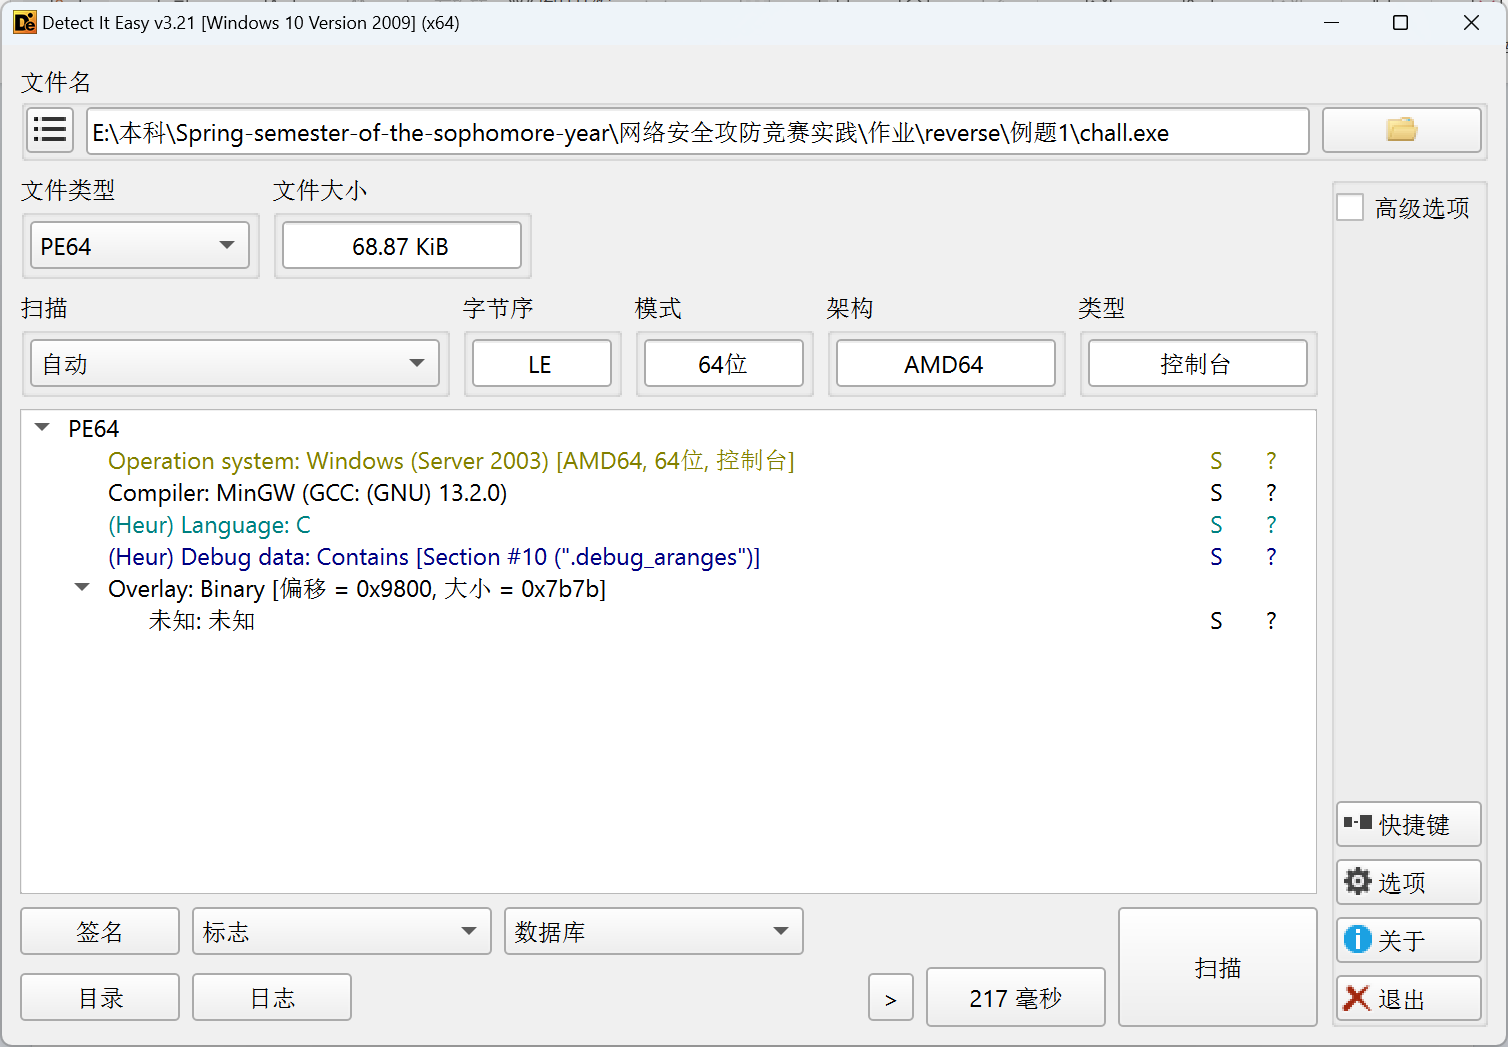
\includegraphics[width=0.95\textwidth]{1.1.png}
    \caption{使用Detect It Easy确认程序为64位无壳PE文件}
\end{figure}

\begin{figure}[H]
    \centering
    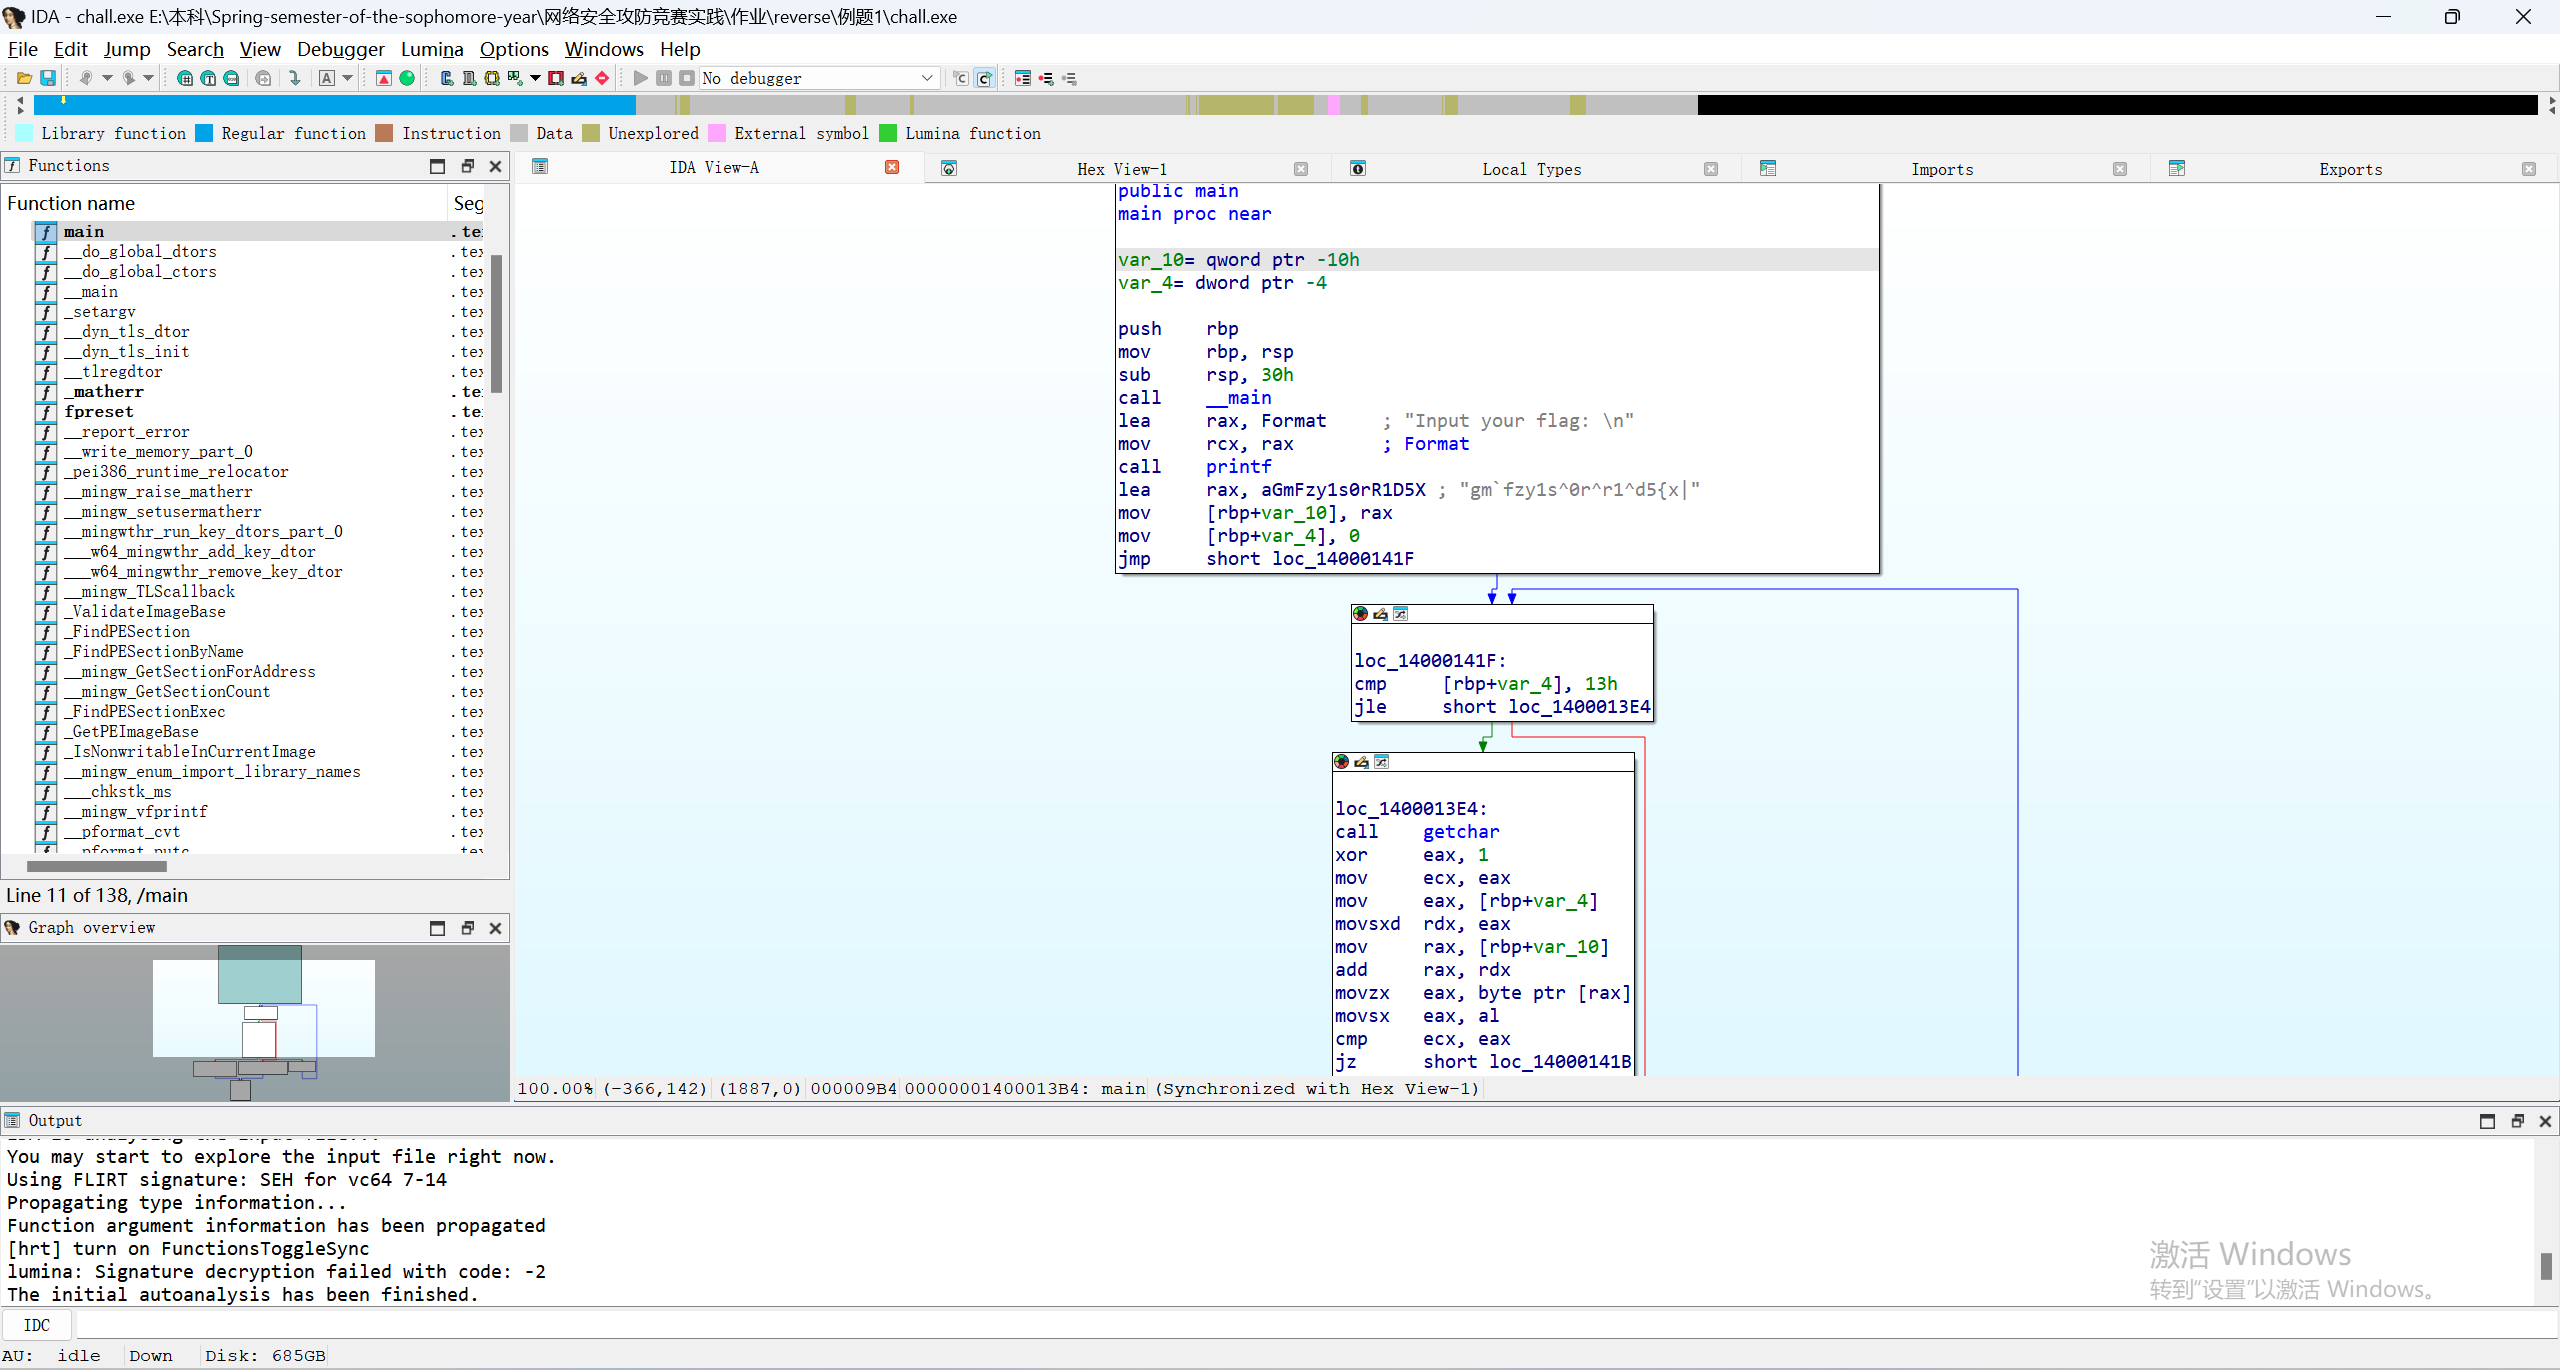
\includegraphics[width=0.95\textwidth]{1.2.png}
    \caption{IDA Pro中查看主函数汇编代码}
\end{figure}

\begin{figure}[H]
    \centering
    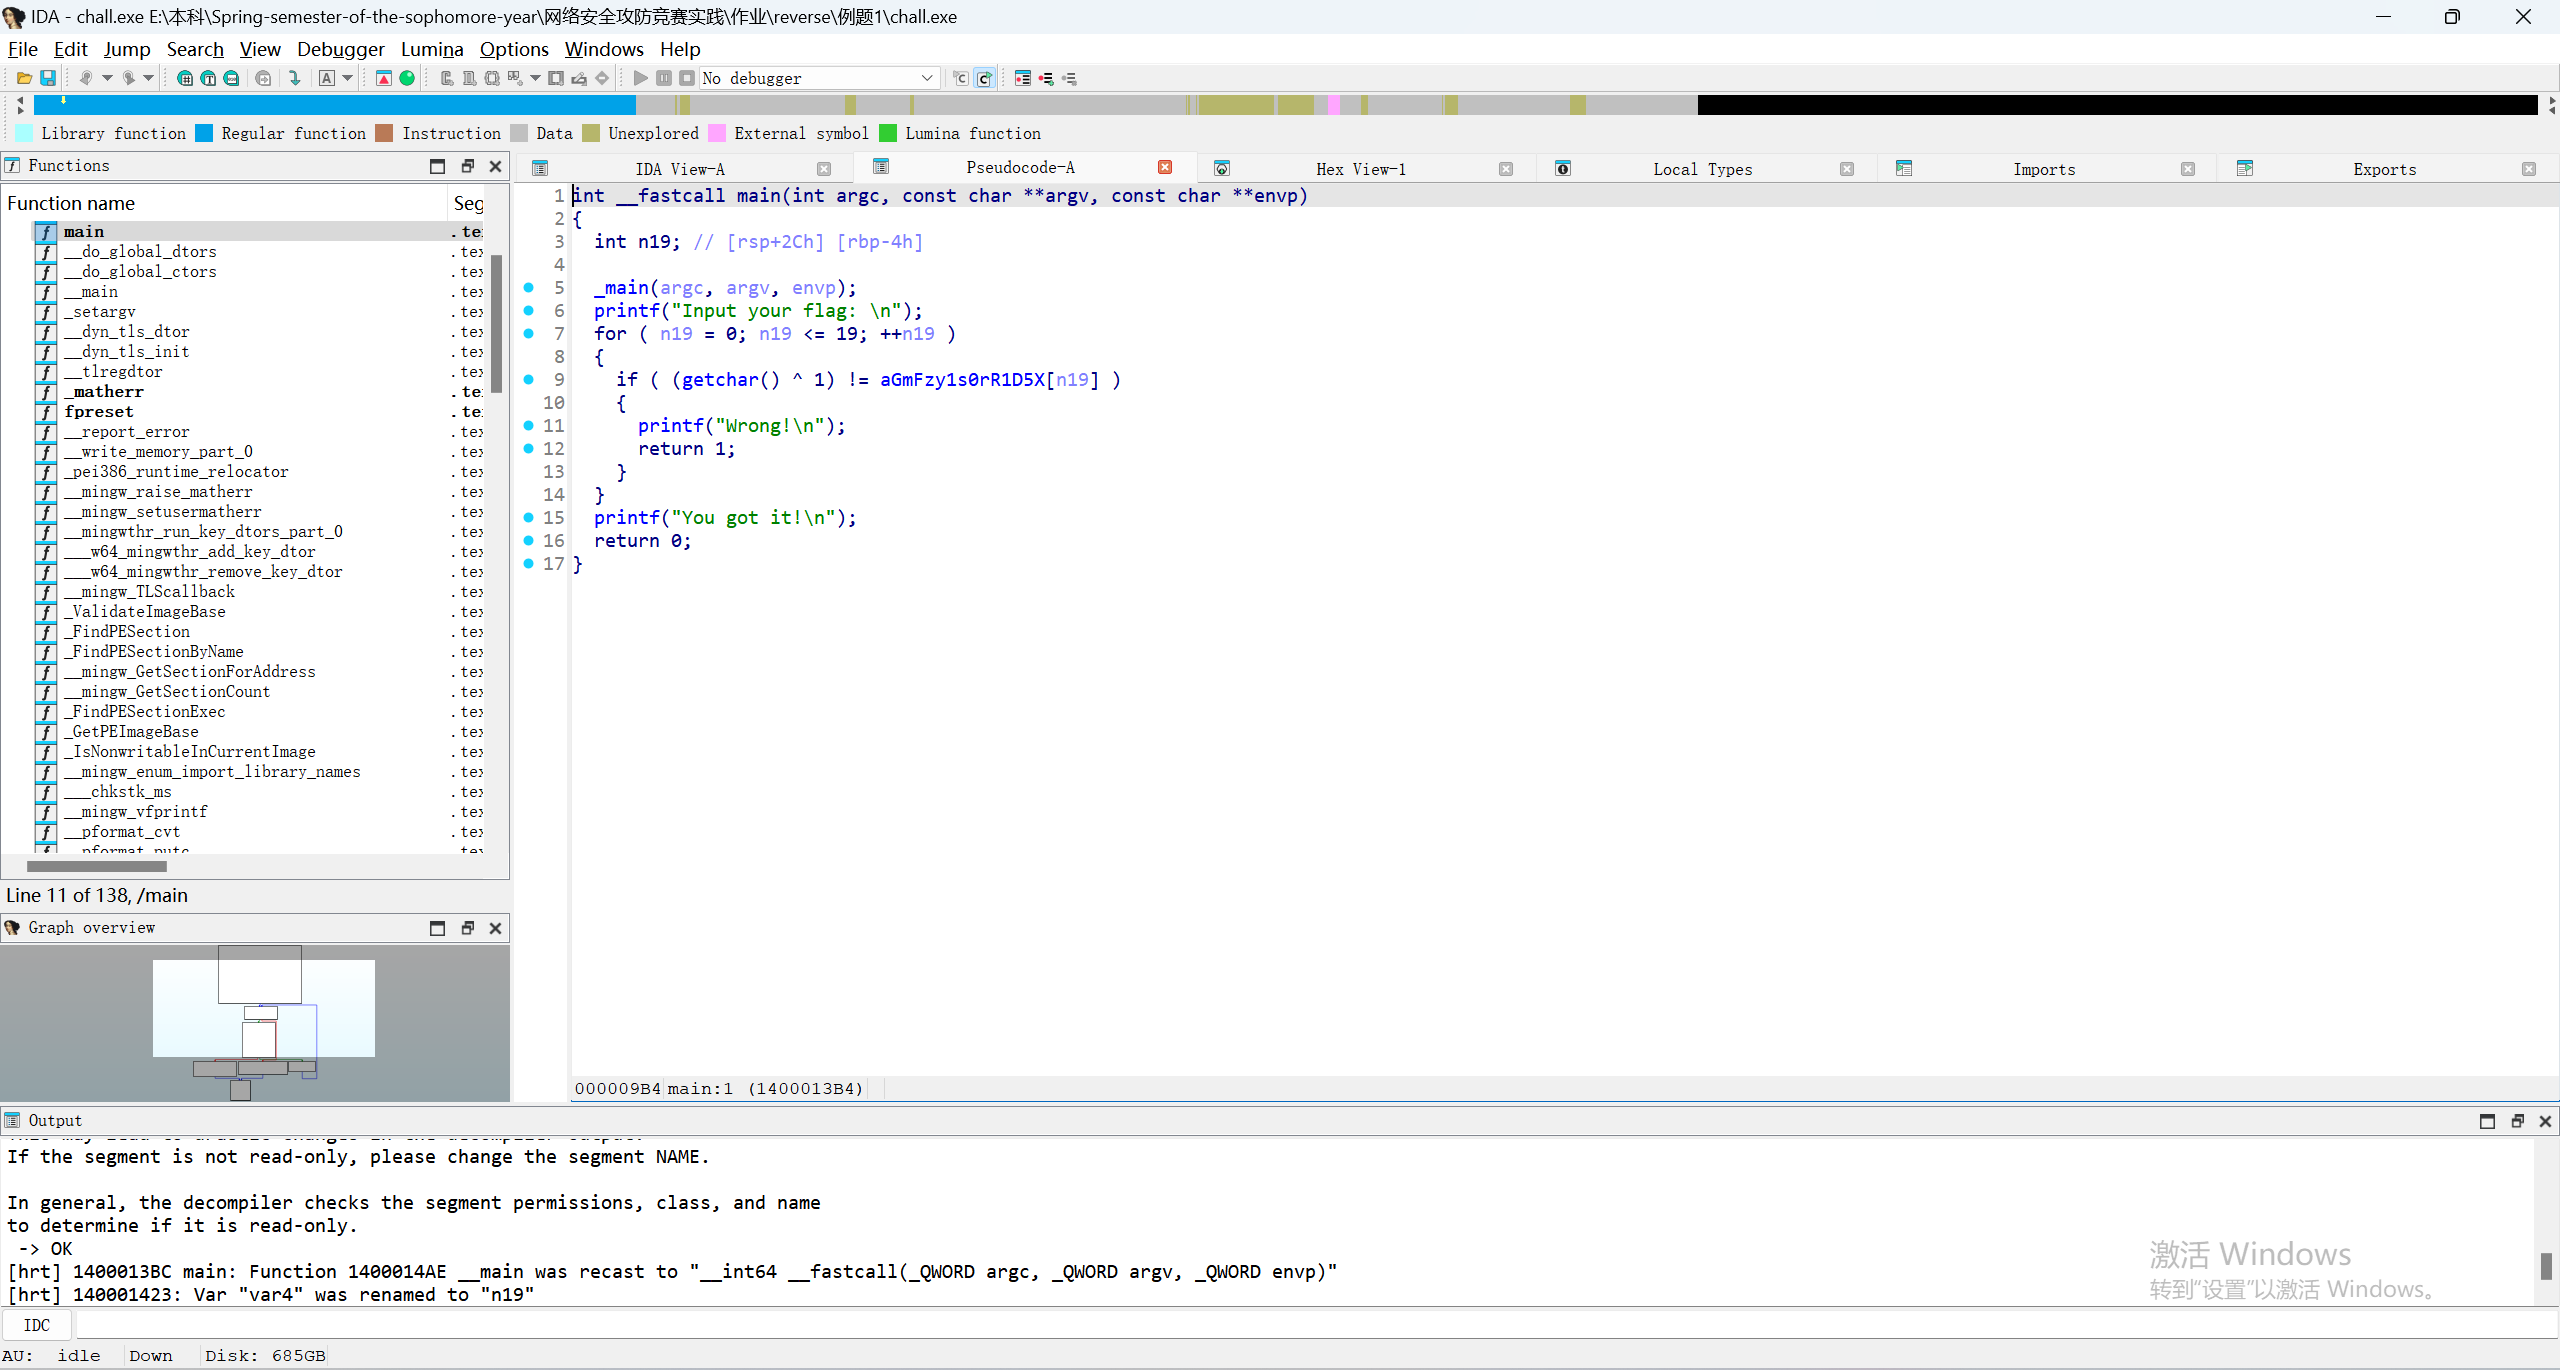
\includegraphics[width=0.95\textwidth]{1.3.png}
    \caption{IDA中查看主函数伪代码，发现异或校验逻辑}
\end{figure}

\begin{figure}[H]
    \centering
    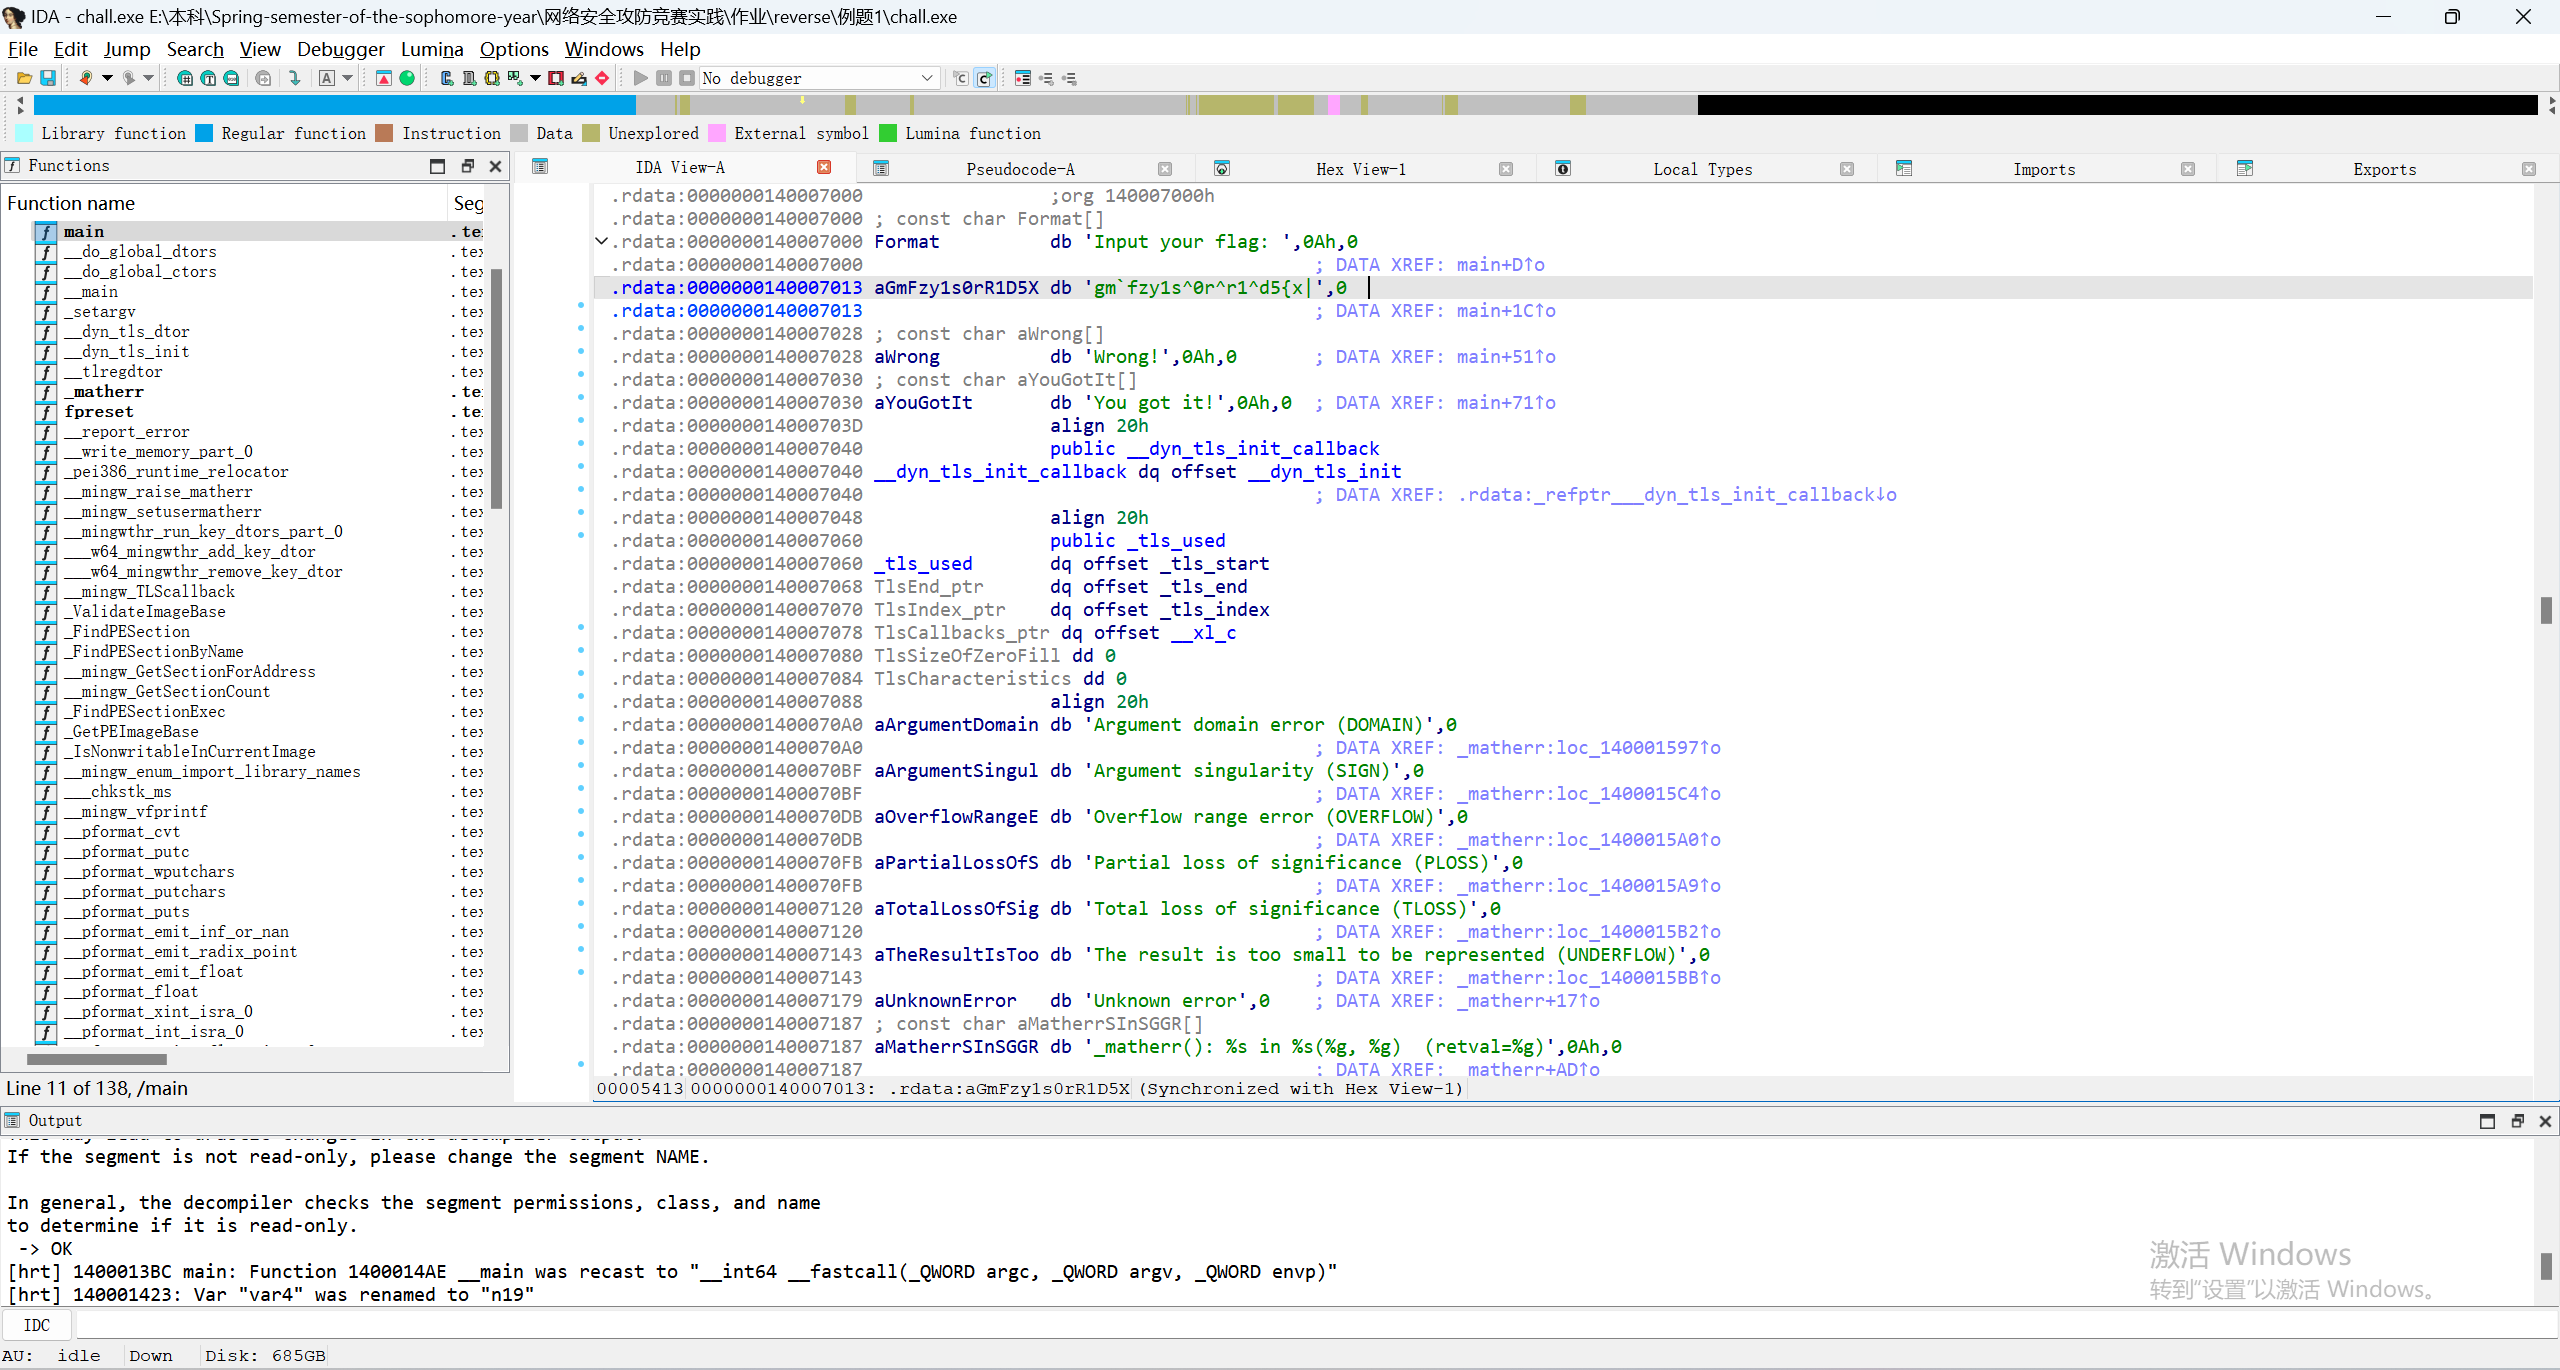
\includegraphics[width=0.95\textwidth]{1.4.png}
    \caption{IDA数据段中查看密文字符串常量}
\end{figure}

\subsubsection{解题脚本与运行结果}
\begin{lstlisting}[language=python]
enc = "gm`fzy1s^0r^r1^d5{x|"
flag = ""
for c in enc:
    flag += chr(ord(c) ^ 0x1)
print("flag{" + flag + "}")
\end{lstlisting}

\begin{figure}[H]
    \centering
    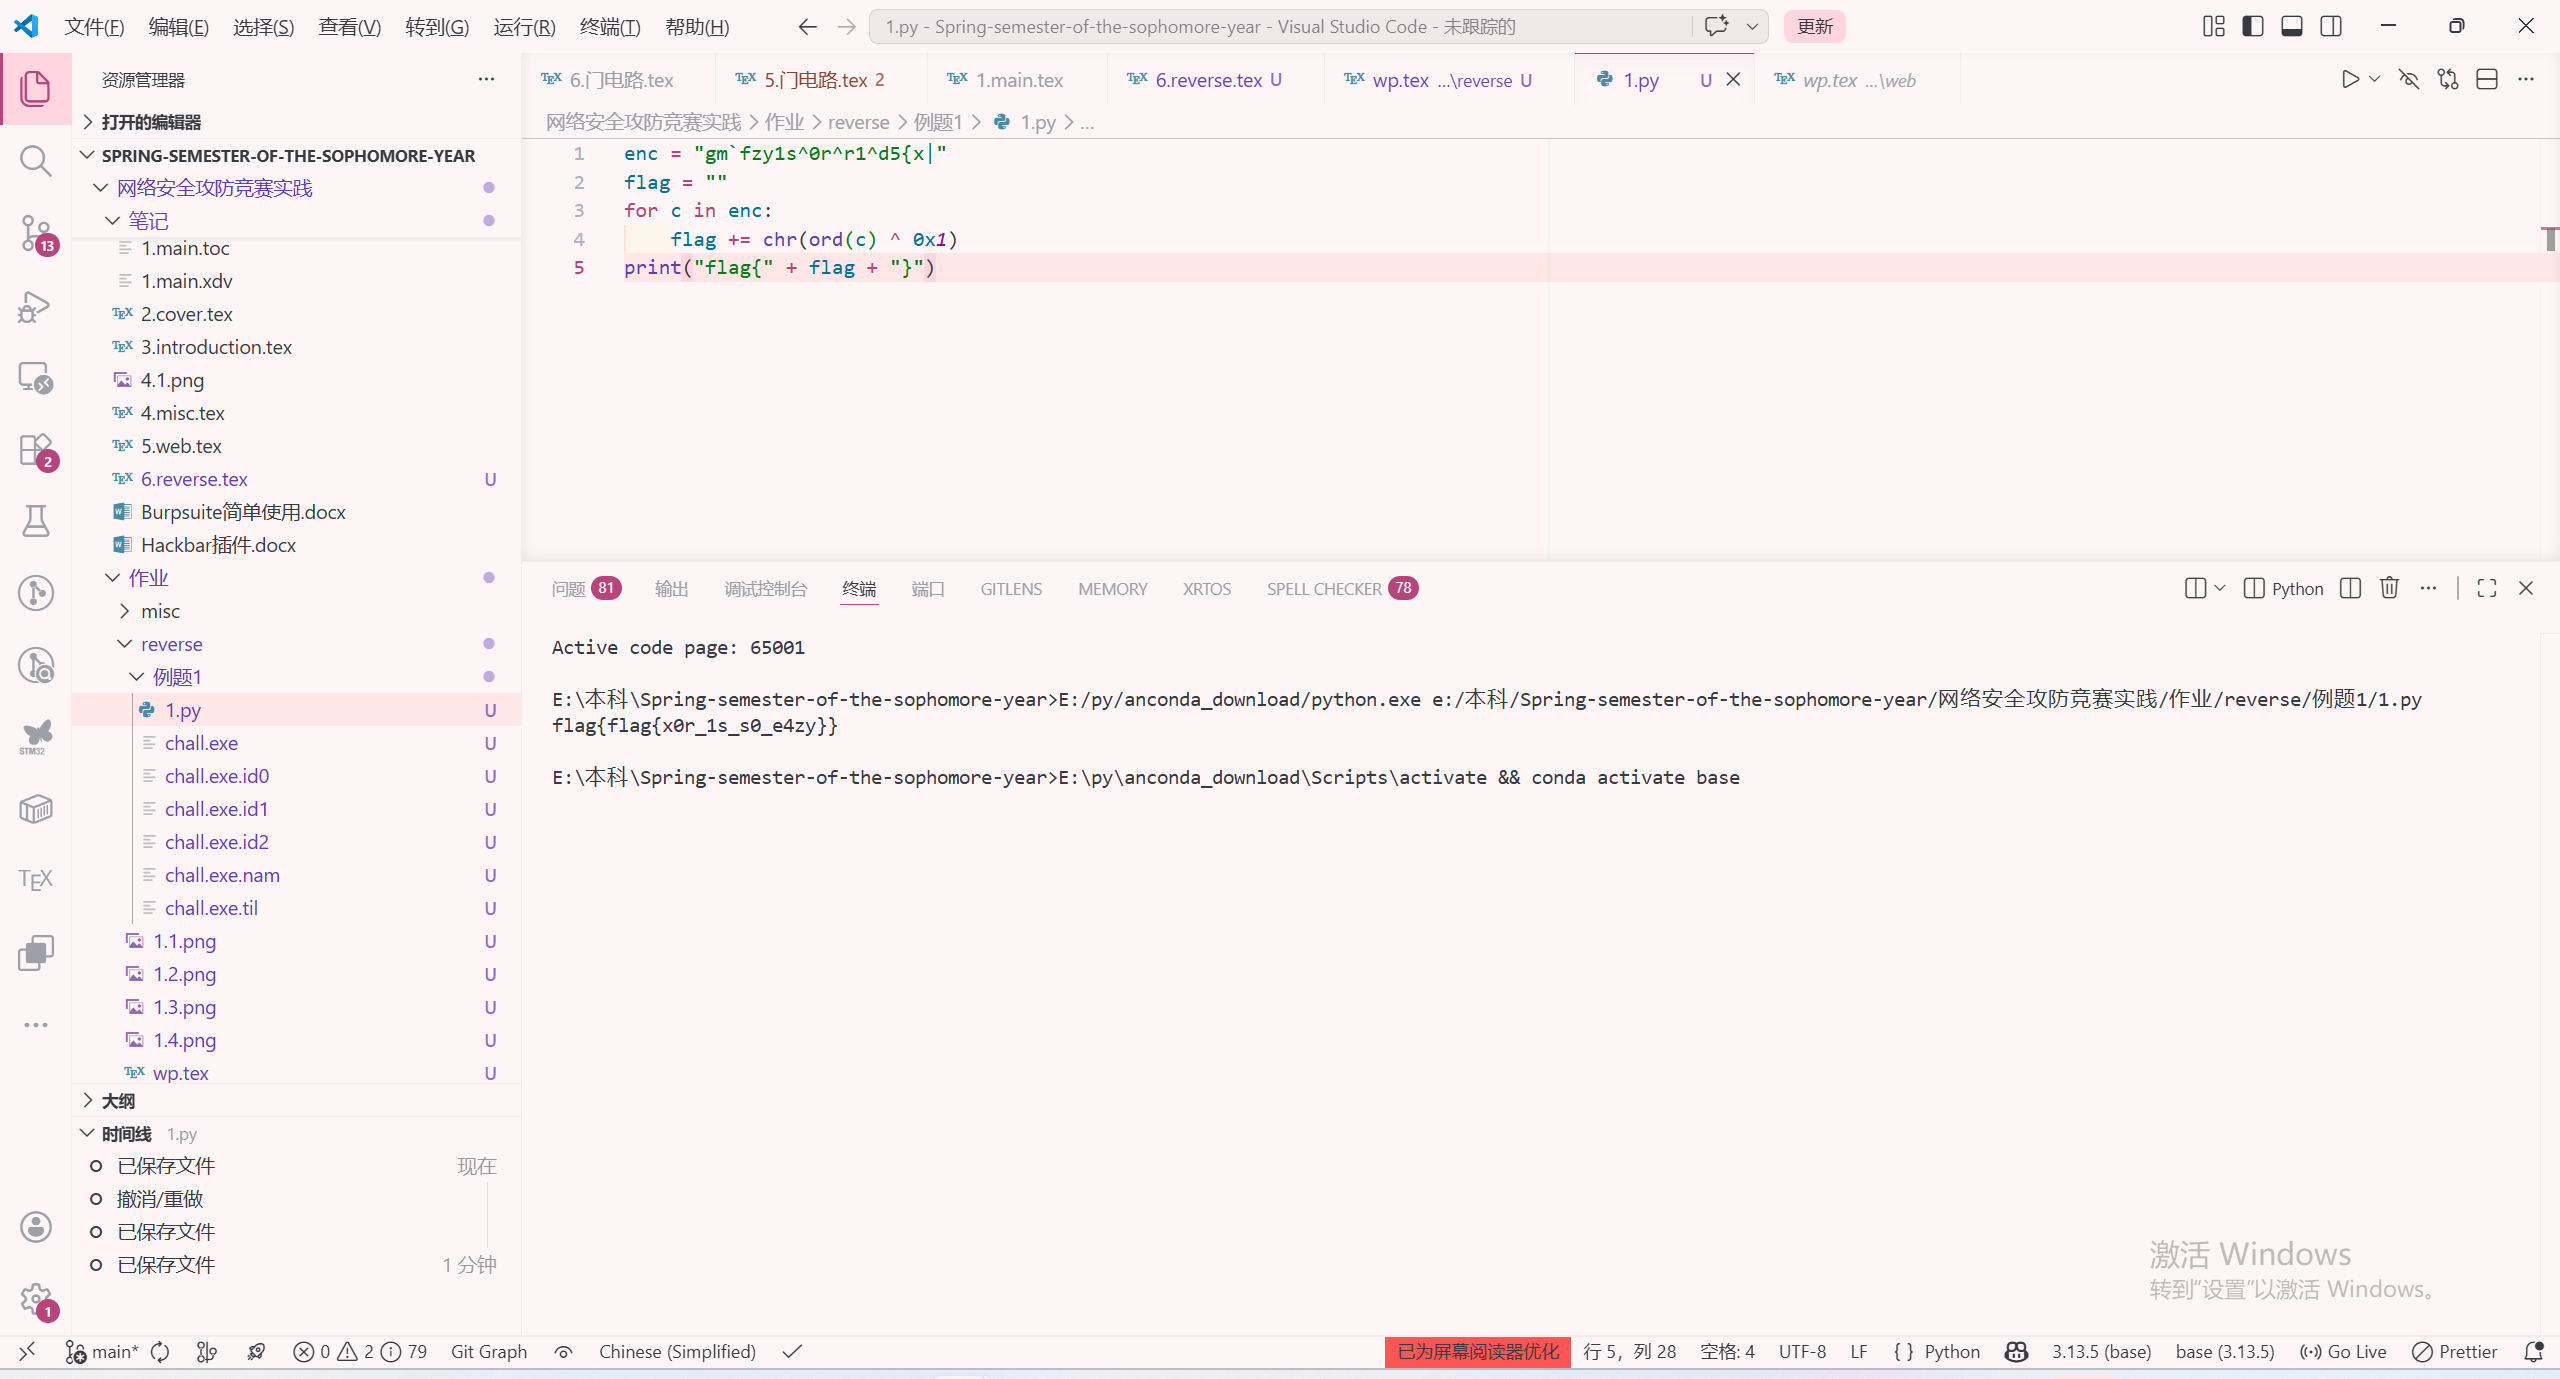
\includegraphics[width=0.95\textwidth]{1.5.png}
\end{figure}

\subsection{最终Flag}
\begin{center}
    \Large flag\{fl0r1s\_e4zy\_is\_x0r\}
\end{center}

\newpage

% --------------------- 题目2：UPX脱壳
\section{题目2：例题-UPX脱壳}
\subsection{题目分析}
本题为逆向工程中典型的UPX壳脱壳例题，核心考察PE文件壳识别、UPX工具手动脱壳、脱壳后程序静态分析的完整流程。程序被标准UPX壳压缩，直接反汇编无法查看有效代码，需先脱壳再分析，脱壳后可直接从主函数中找到明文flag。

\subsection{解题步骤}
\begin{enumerate}
    \item 使用 Detect It Easy (DiE) 工具分析 \texttt{chall.exe}，确认文件为64位PE可执行文件，被UPX(4.23)[NRV.best]壳压缩。
    \item 使用 UPX 工具执行脱壳命令：\texttt{upx.exe -d chall.exe}，完成自动脱壳。
    \item 脱壳完成后，再次使用 DiE 扫描文件，确认UPX壳已被移除，程序恢复为无壳状态。
    \item 使用 IDA Pro 64位加载脱壳后的程序，直接查看主函数汇编代码，即可找到明文flag字符串。
\end{enumerate}

\begin{figure}[H]
    \centering
    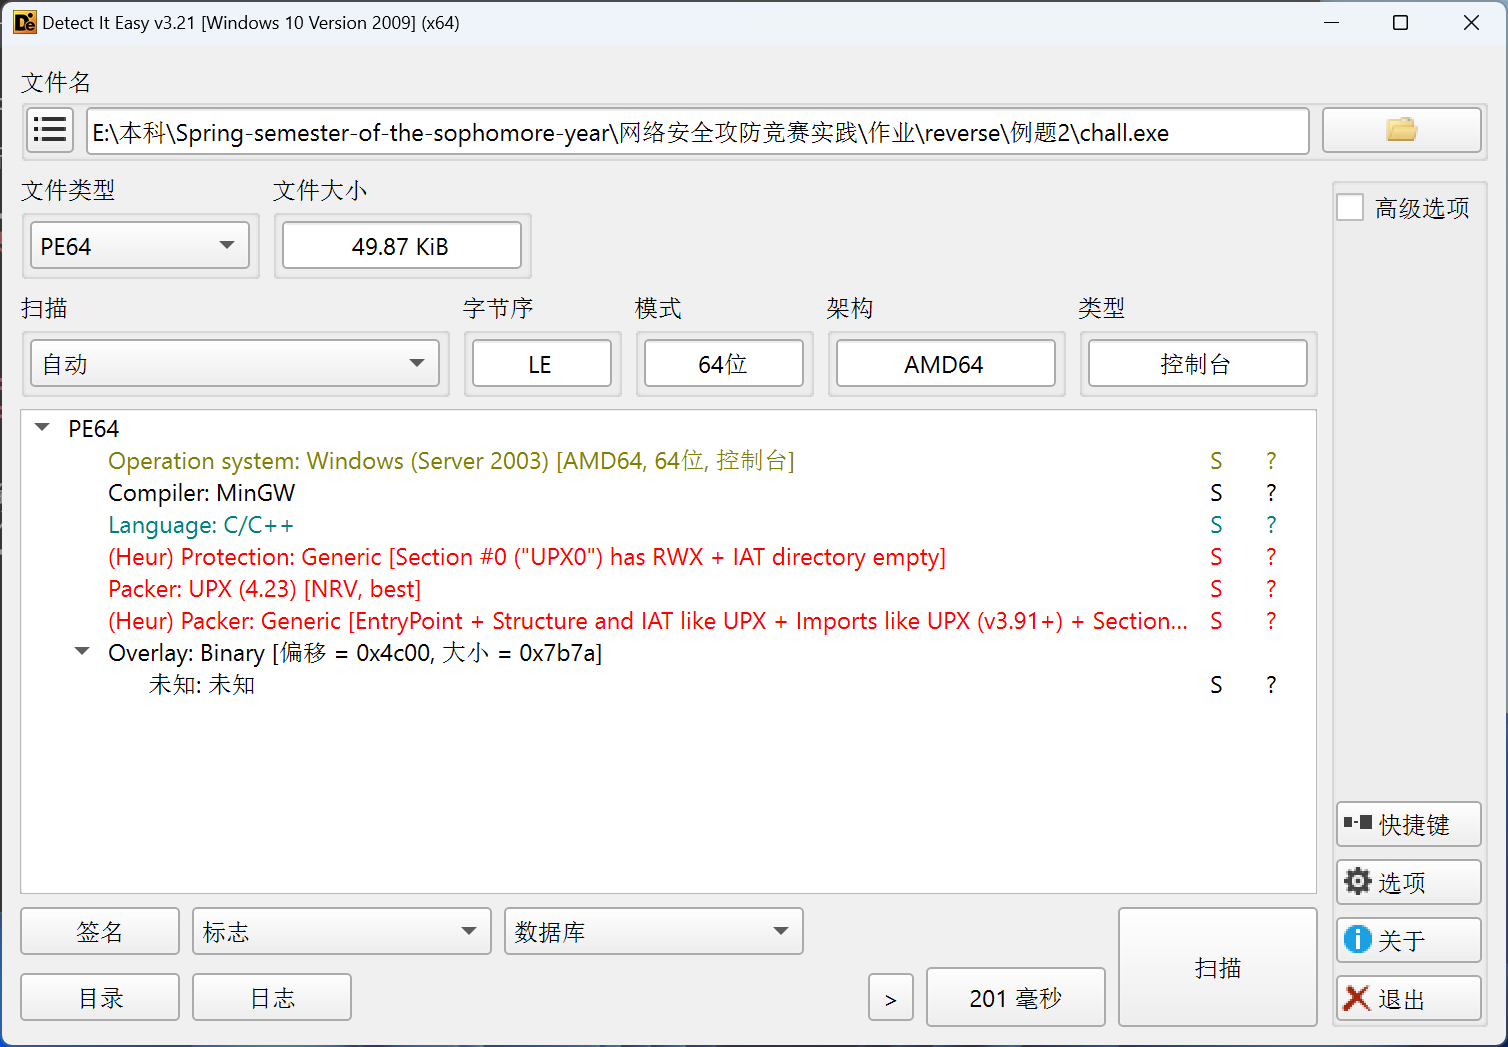
\includegraphics[width=0.95\textwidth]{2.1.png}
\end{figure}
\begin{figure}[H]
    \centering
    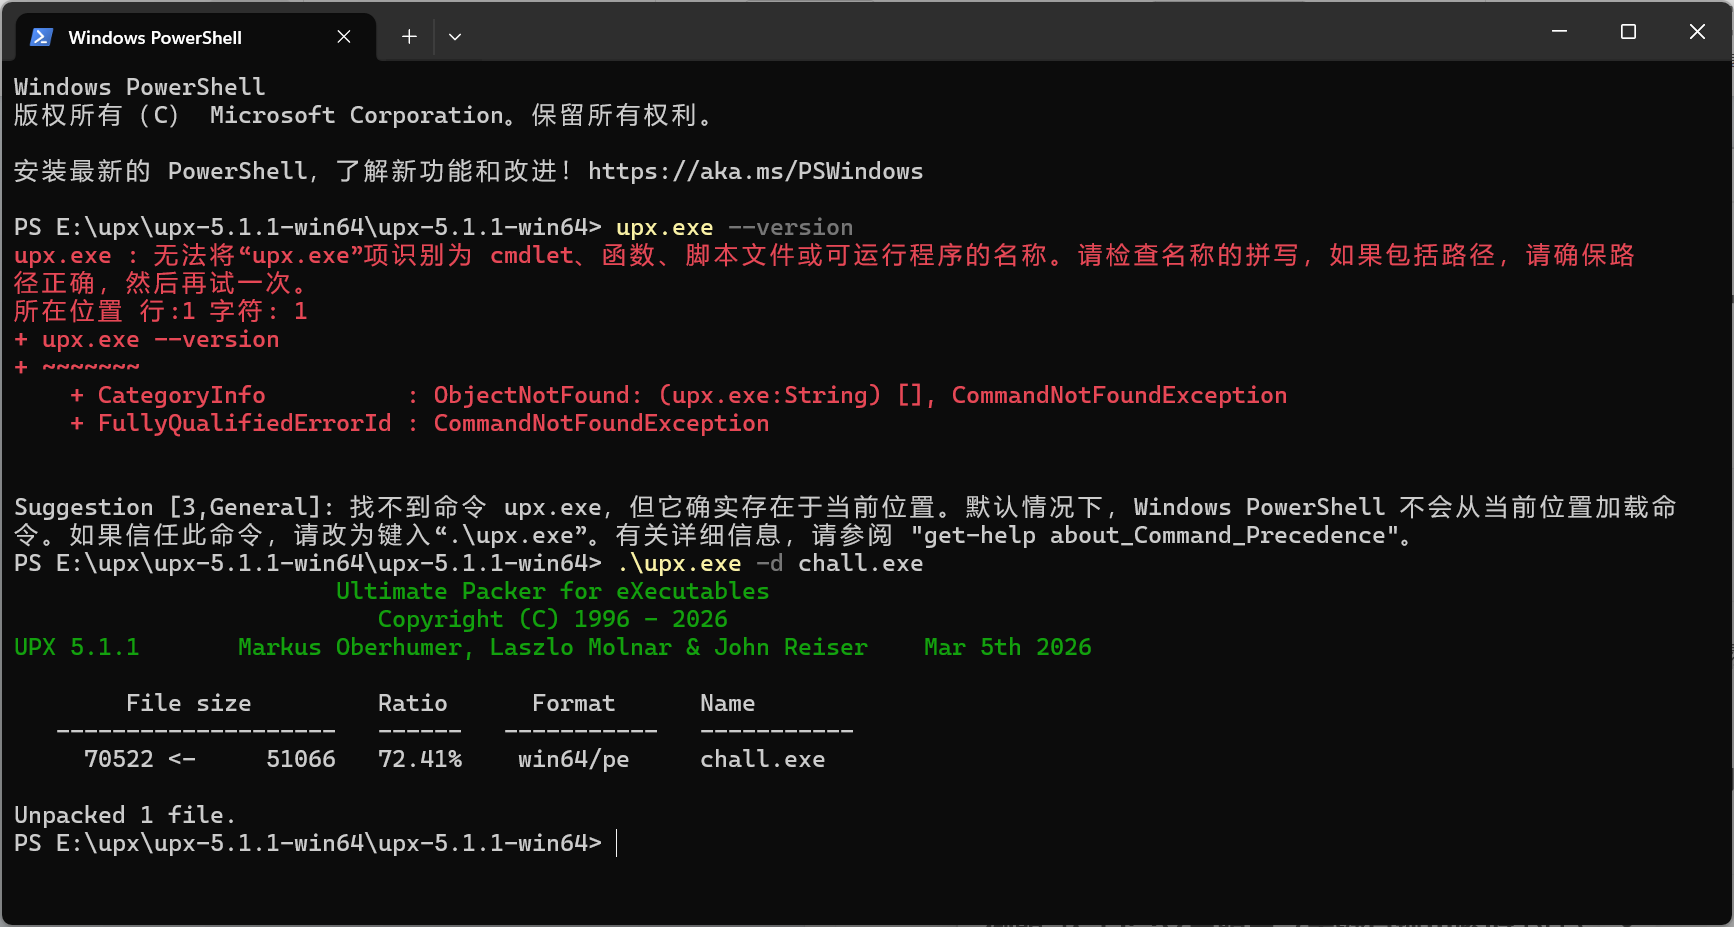
\includegraphics[width=0.95\textwidth]{2.2.png}
\end{figure}
\begin{figure}[H]
    \centering
    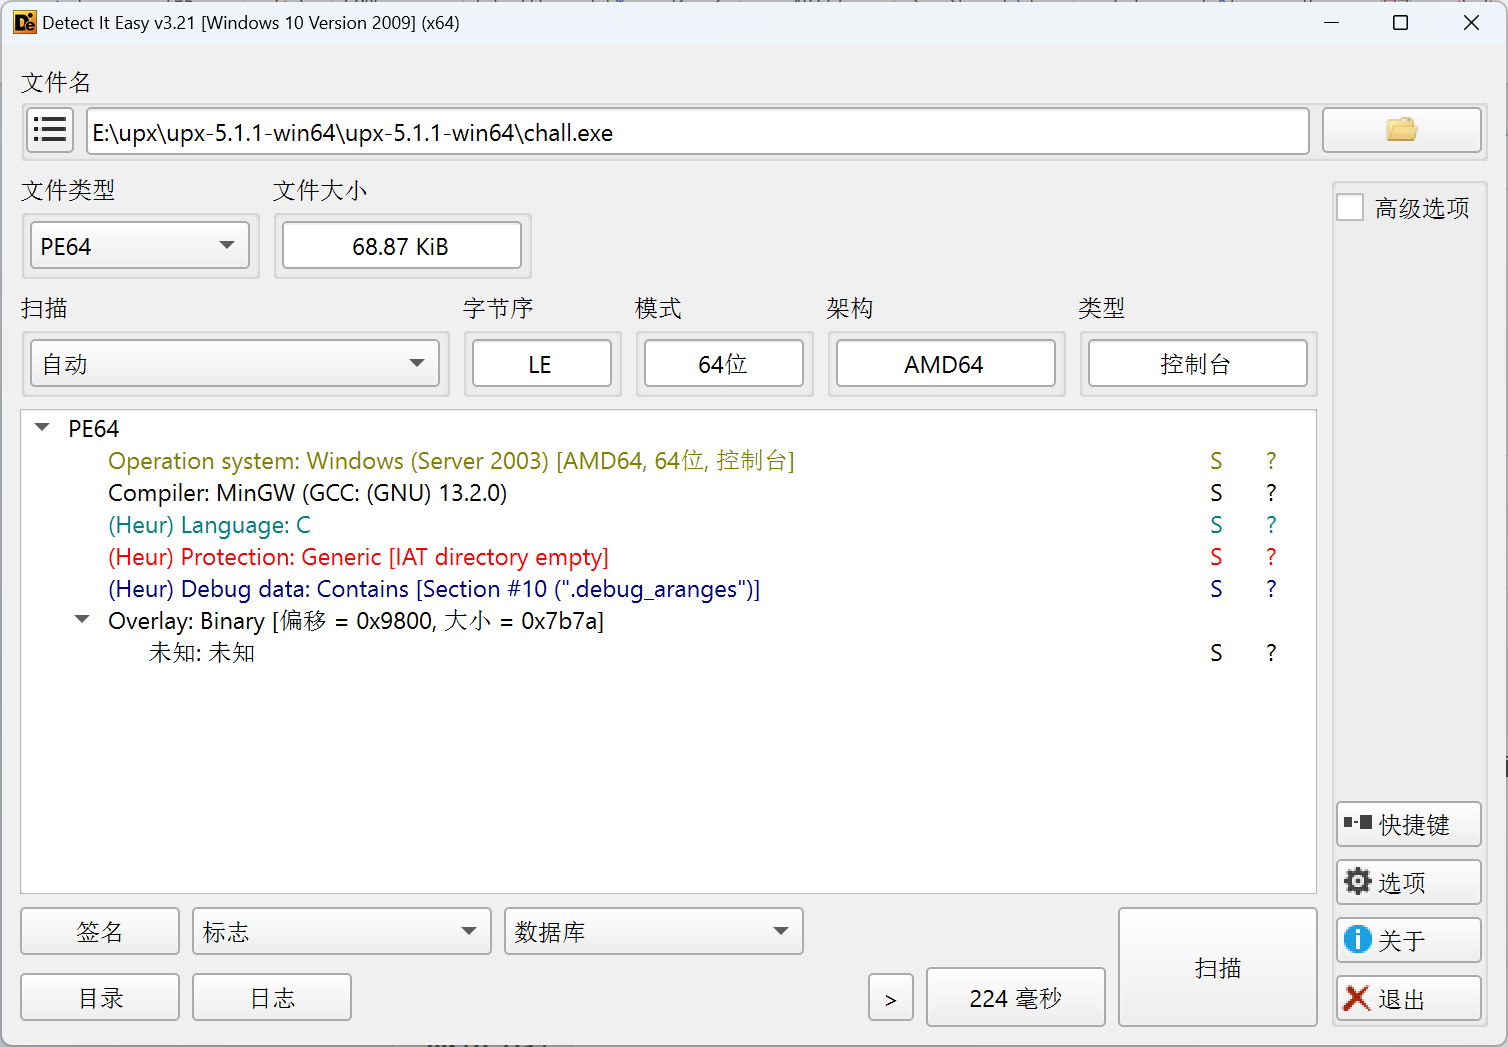
\includegraphics[width=0.95\textwidth]{2.3.png}
\end{figure}
\begin{figure}[H]
    \centering
    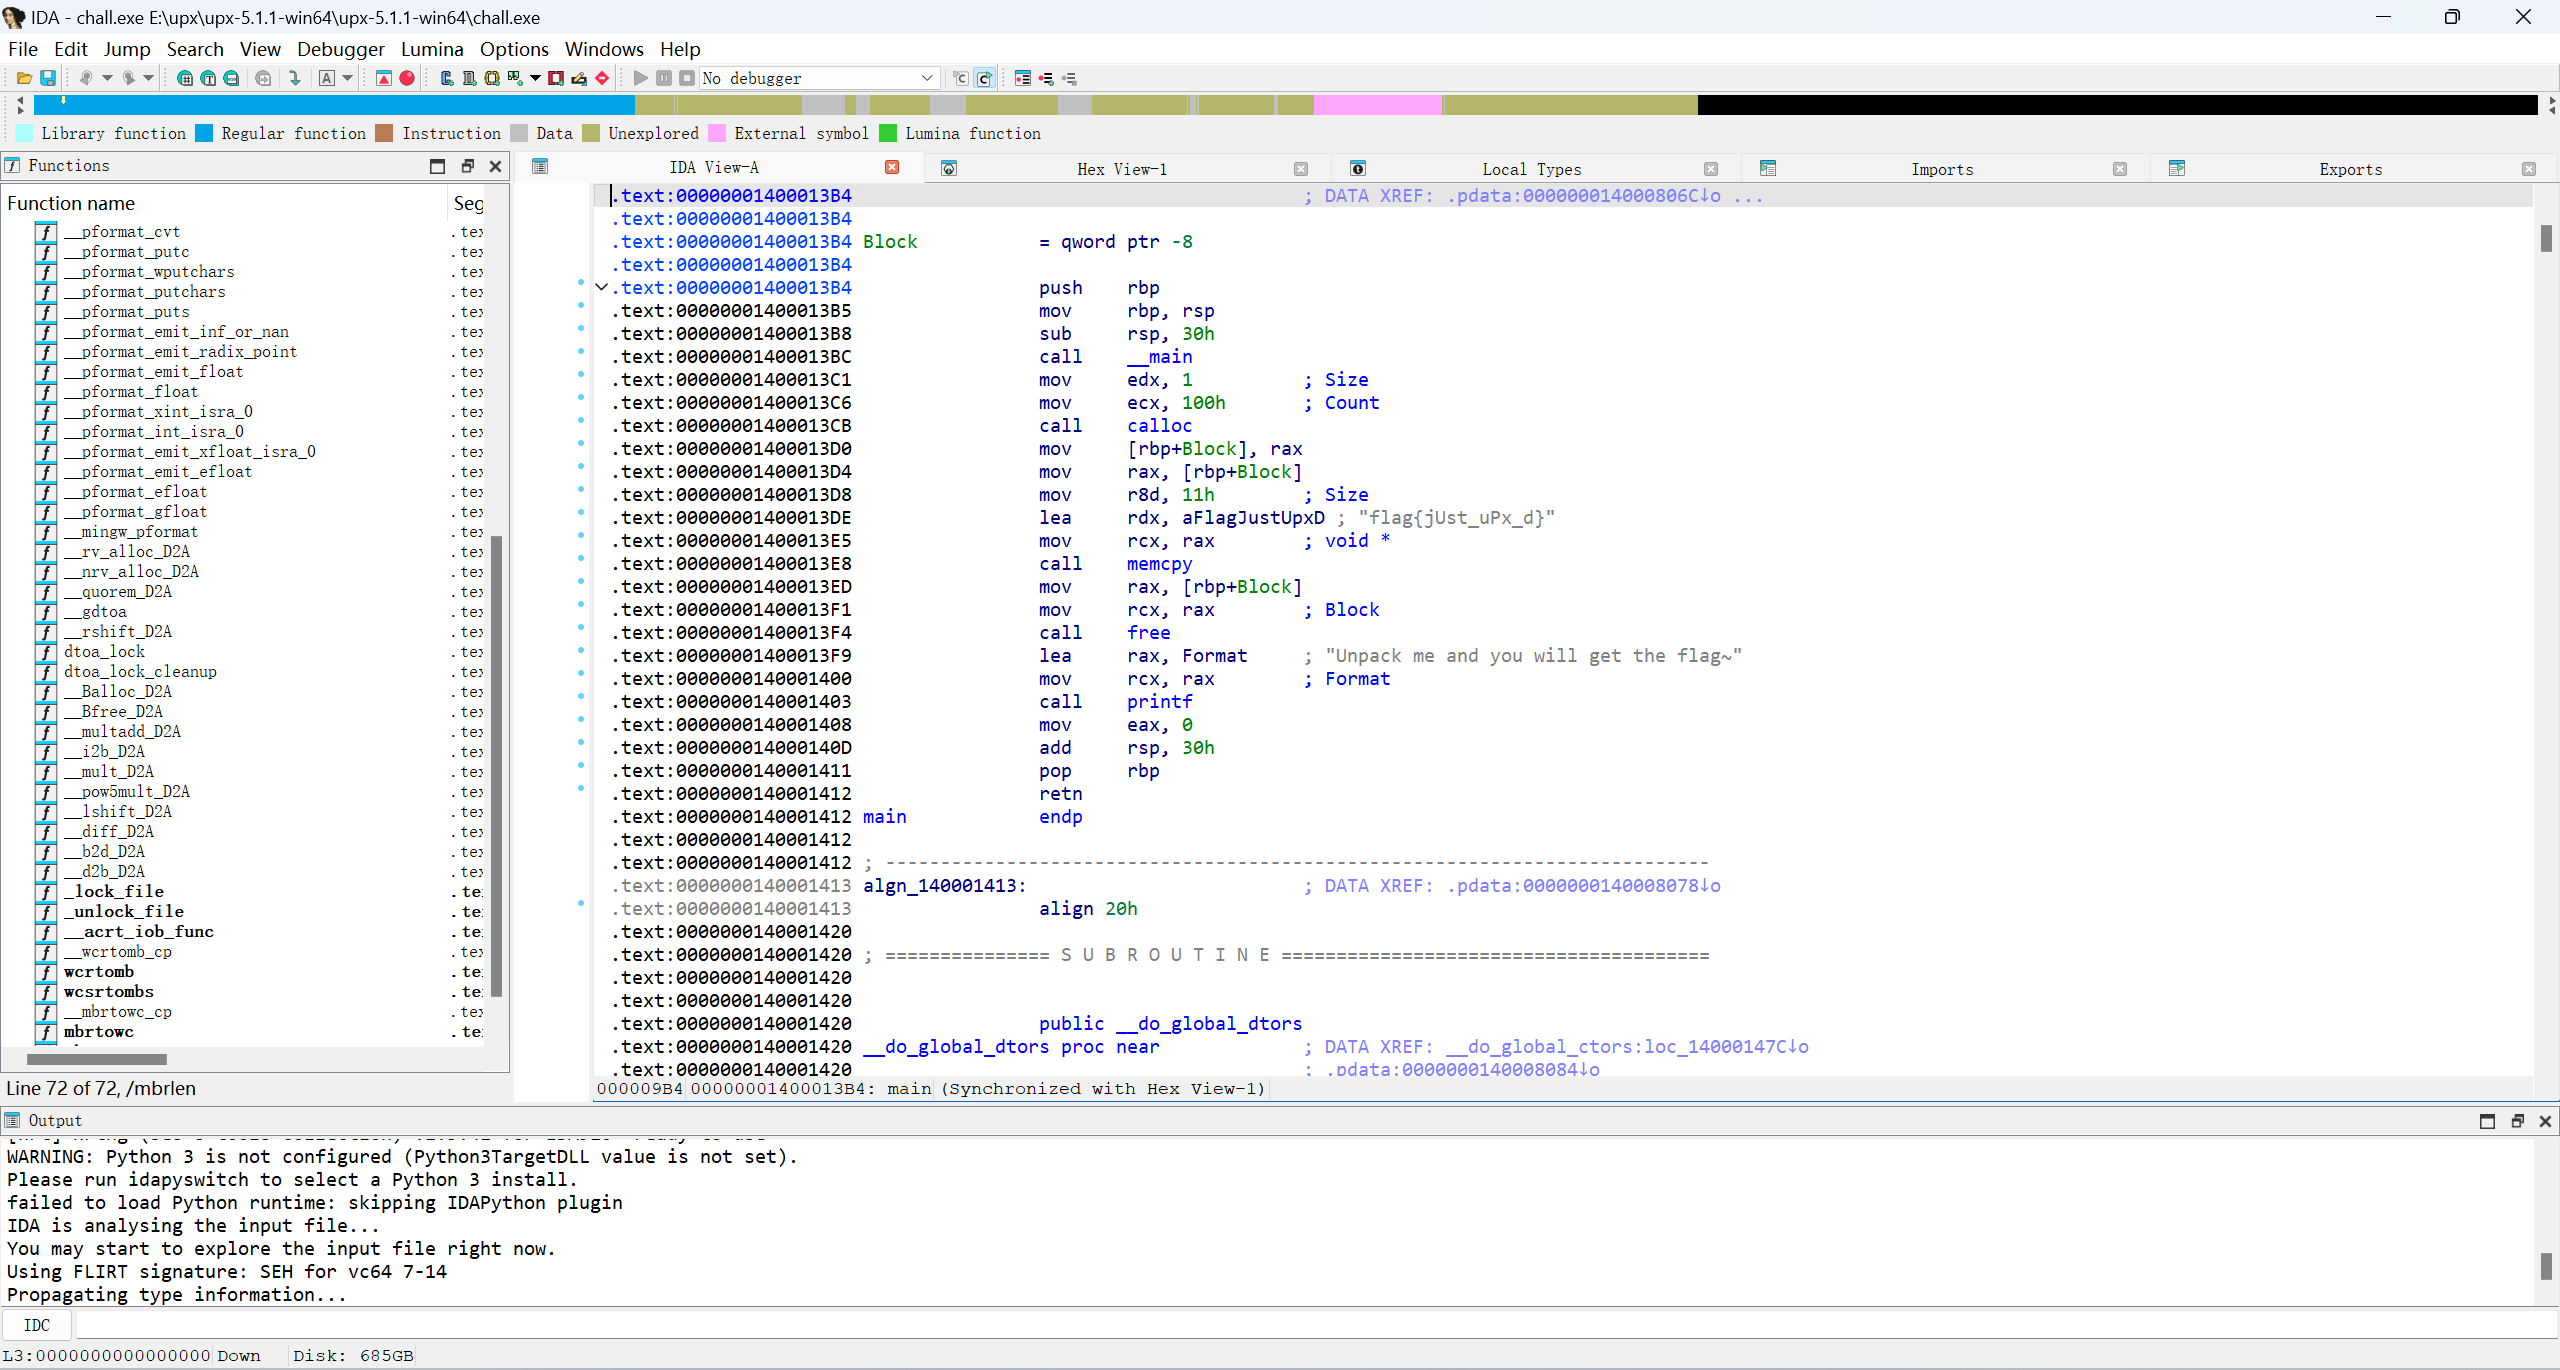
\includegraphics[width=0.95\textwidth]{2.4.png}
\end{figure}

\subsection{最终Flag}
\begin{center}
    \Large flag\{jUst\_uPx\_d\}
\end{center}

\newpage

% --------------------- 题目3：自定义壳脱壳
\section{题目3：例题-自定义壳脱壳}
\subsection{题目分析}
本题属于自定义壳动态加载逆向，无常规PE壳特征，静态分析无法得到有效逻辑。程序运行时会解密释放临时DLL文件，执行完核心逻辑后调用删除接口清理临时文件，需要借助IDA动态调试断点拦截，在文件删除前抓取DLL再静态分析获取flag。

\subsection{解题步骤}
\begin{enumerate}
    \item 使用 Detect It Easy 检测程序，无标准UPX壳及常见壳特征，判定为自定义壳保护。
    \item IDA 载入程序，F5 反编译伪代码，观察到程序生成并加载 \texttt{.temp.dll}，最后调用 \texttt{remove} 删除临时文件。
    \item 在 \texttt{remove(FileName)} 语句行设置断点，选择本地Windows调试器启动调试。
    \item 程序断下时，临时DLL已生成尚未删除，立刻复制备份该DLL文件。
    \item 使用 IDA 载入备份的 \texttt{.temp.dll}，静态分析即可得到明文flag。
\end{enumerate}

\begin{figure}[H]
    \centering
    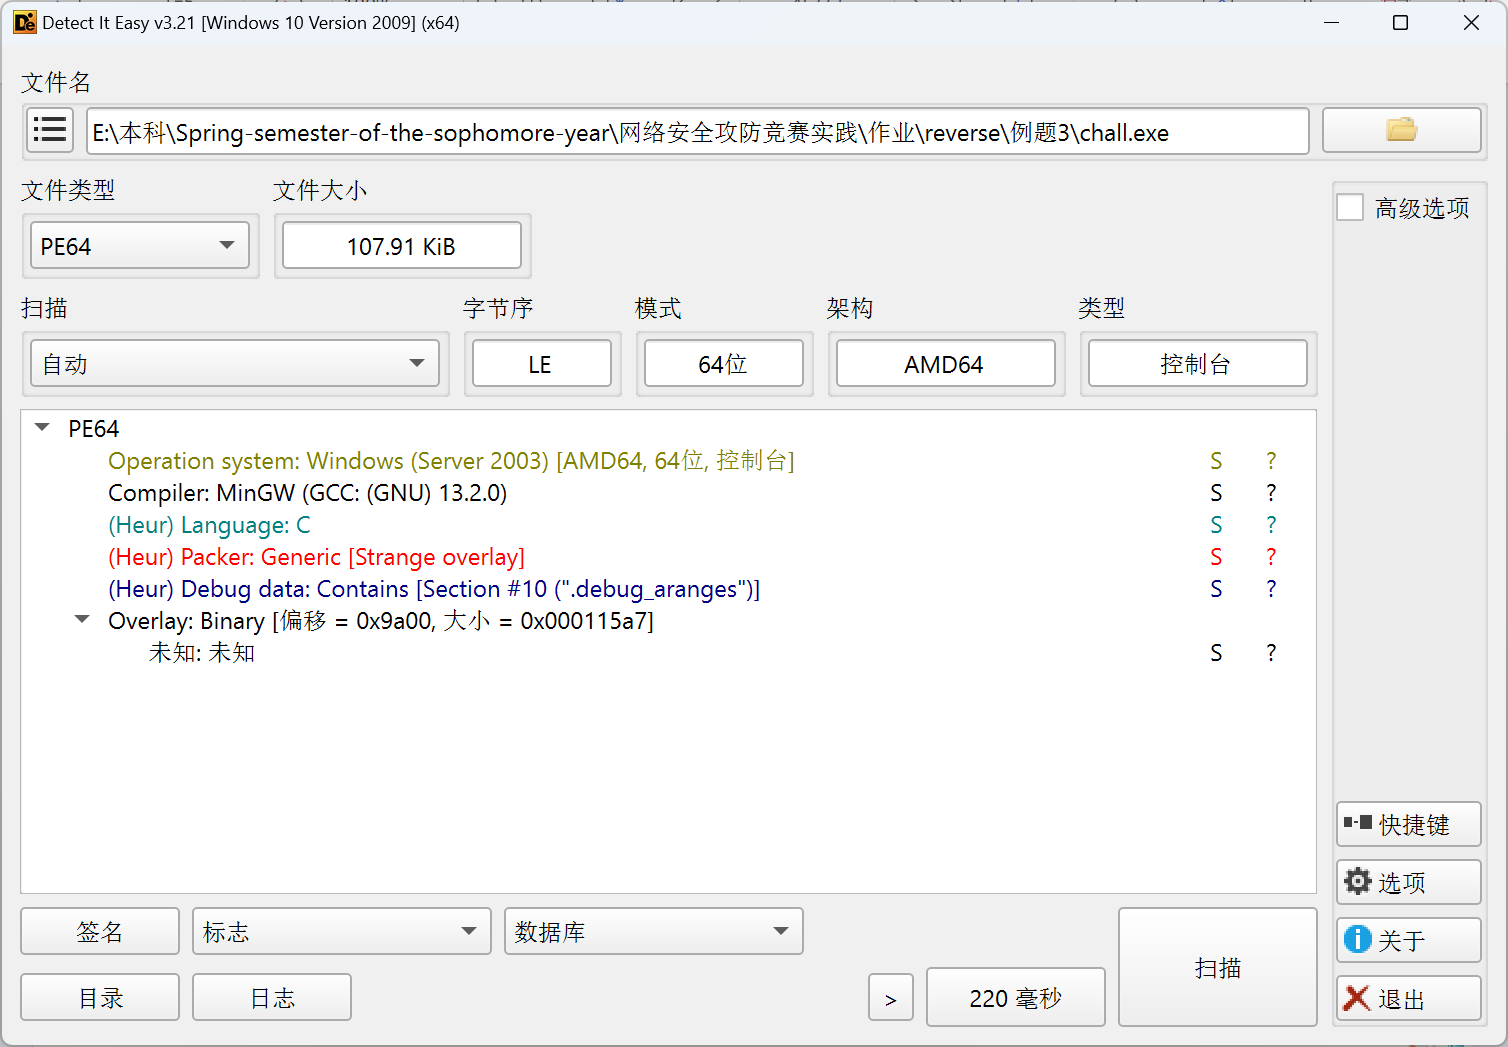
\includegraphics[width=0.95\textwidth]{3.1.png}
\end{figure}
\begin{figure}[H]
    \centering
    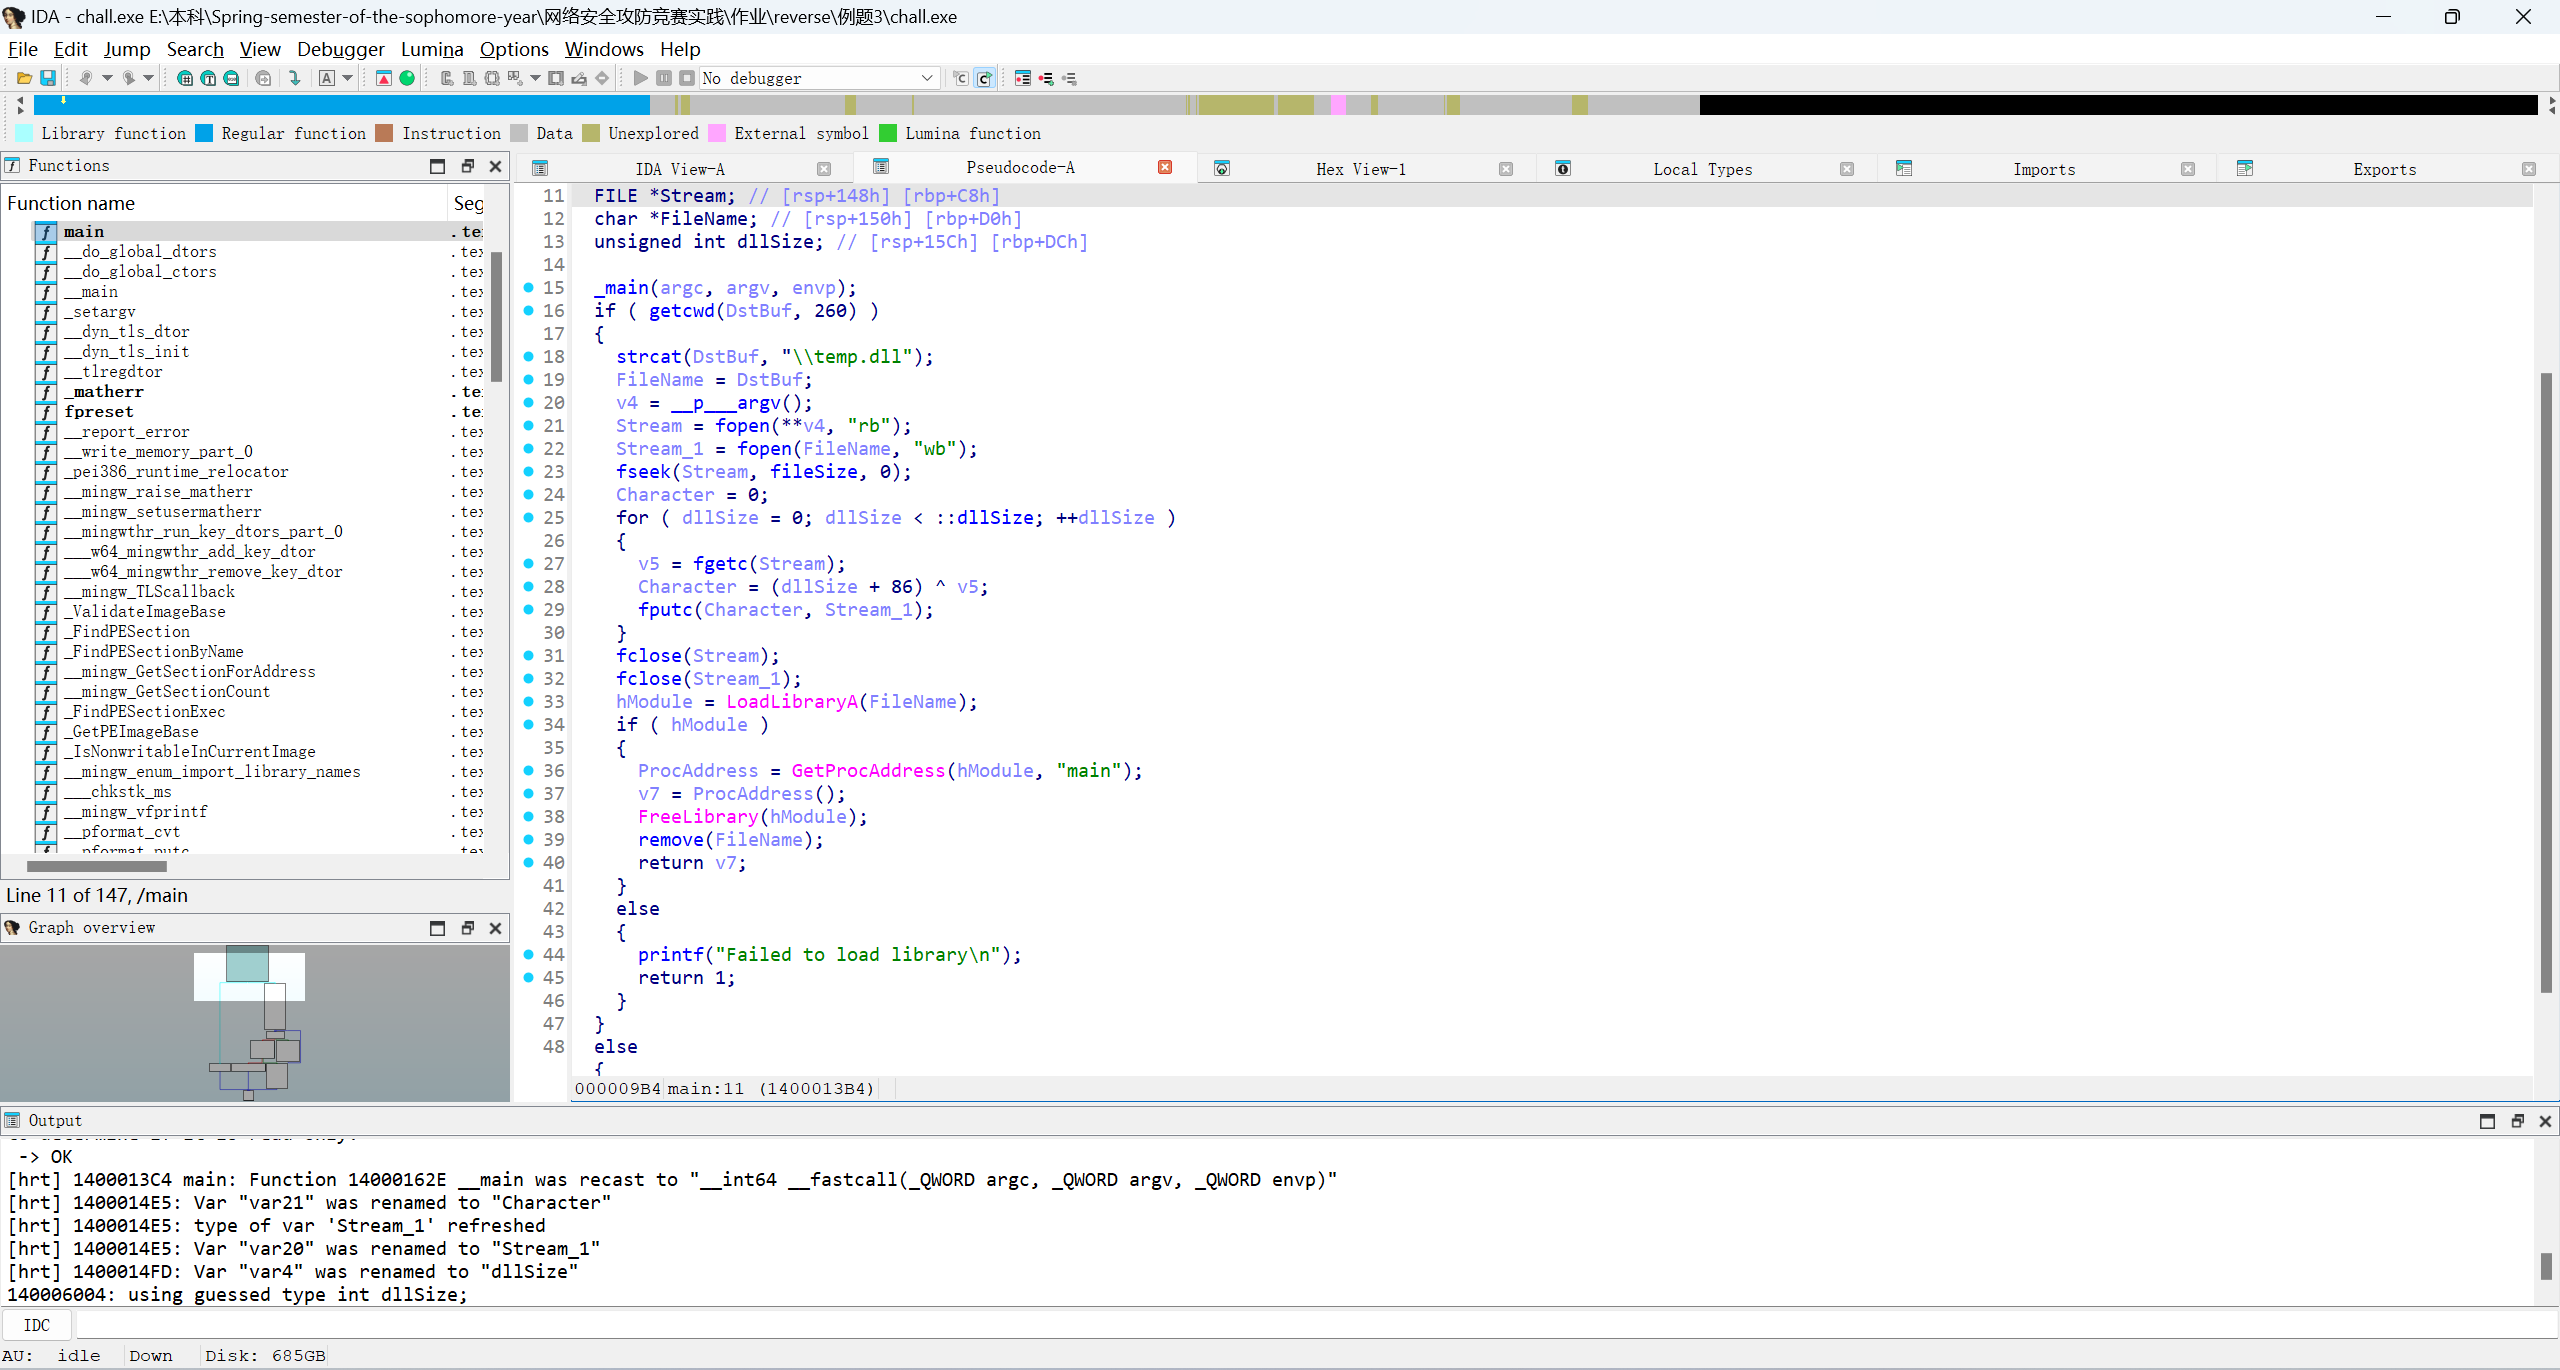
\includegraphics[width=0.95\textwidth]{3.2.png}
\end{figure}
\begin{figure}[H]
    \centering
    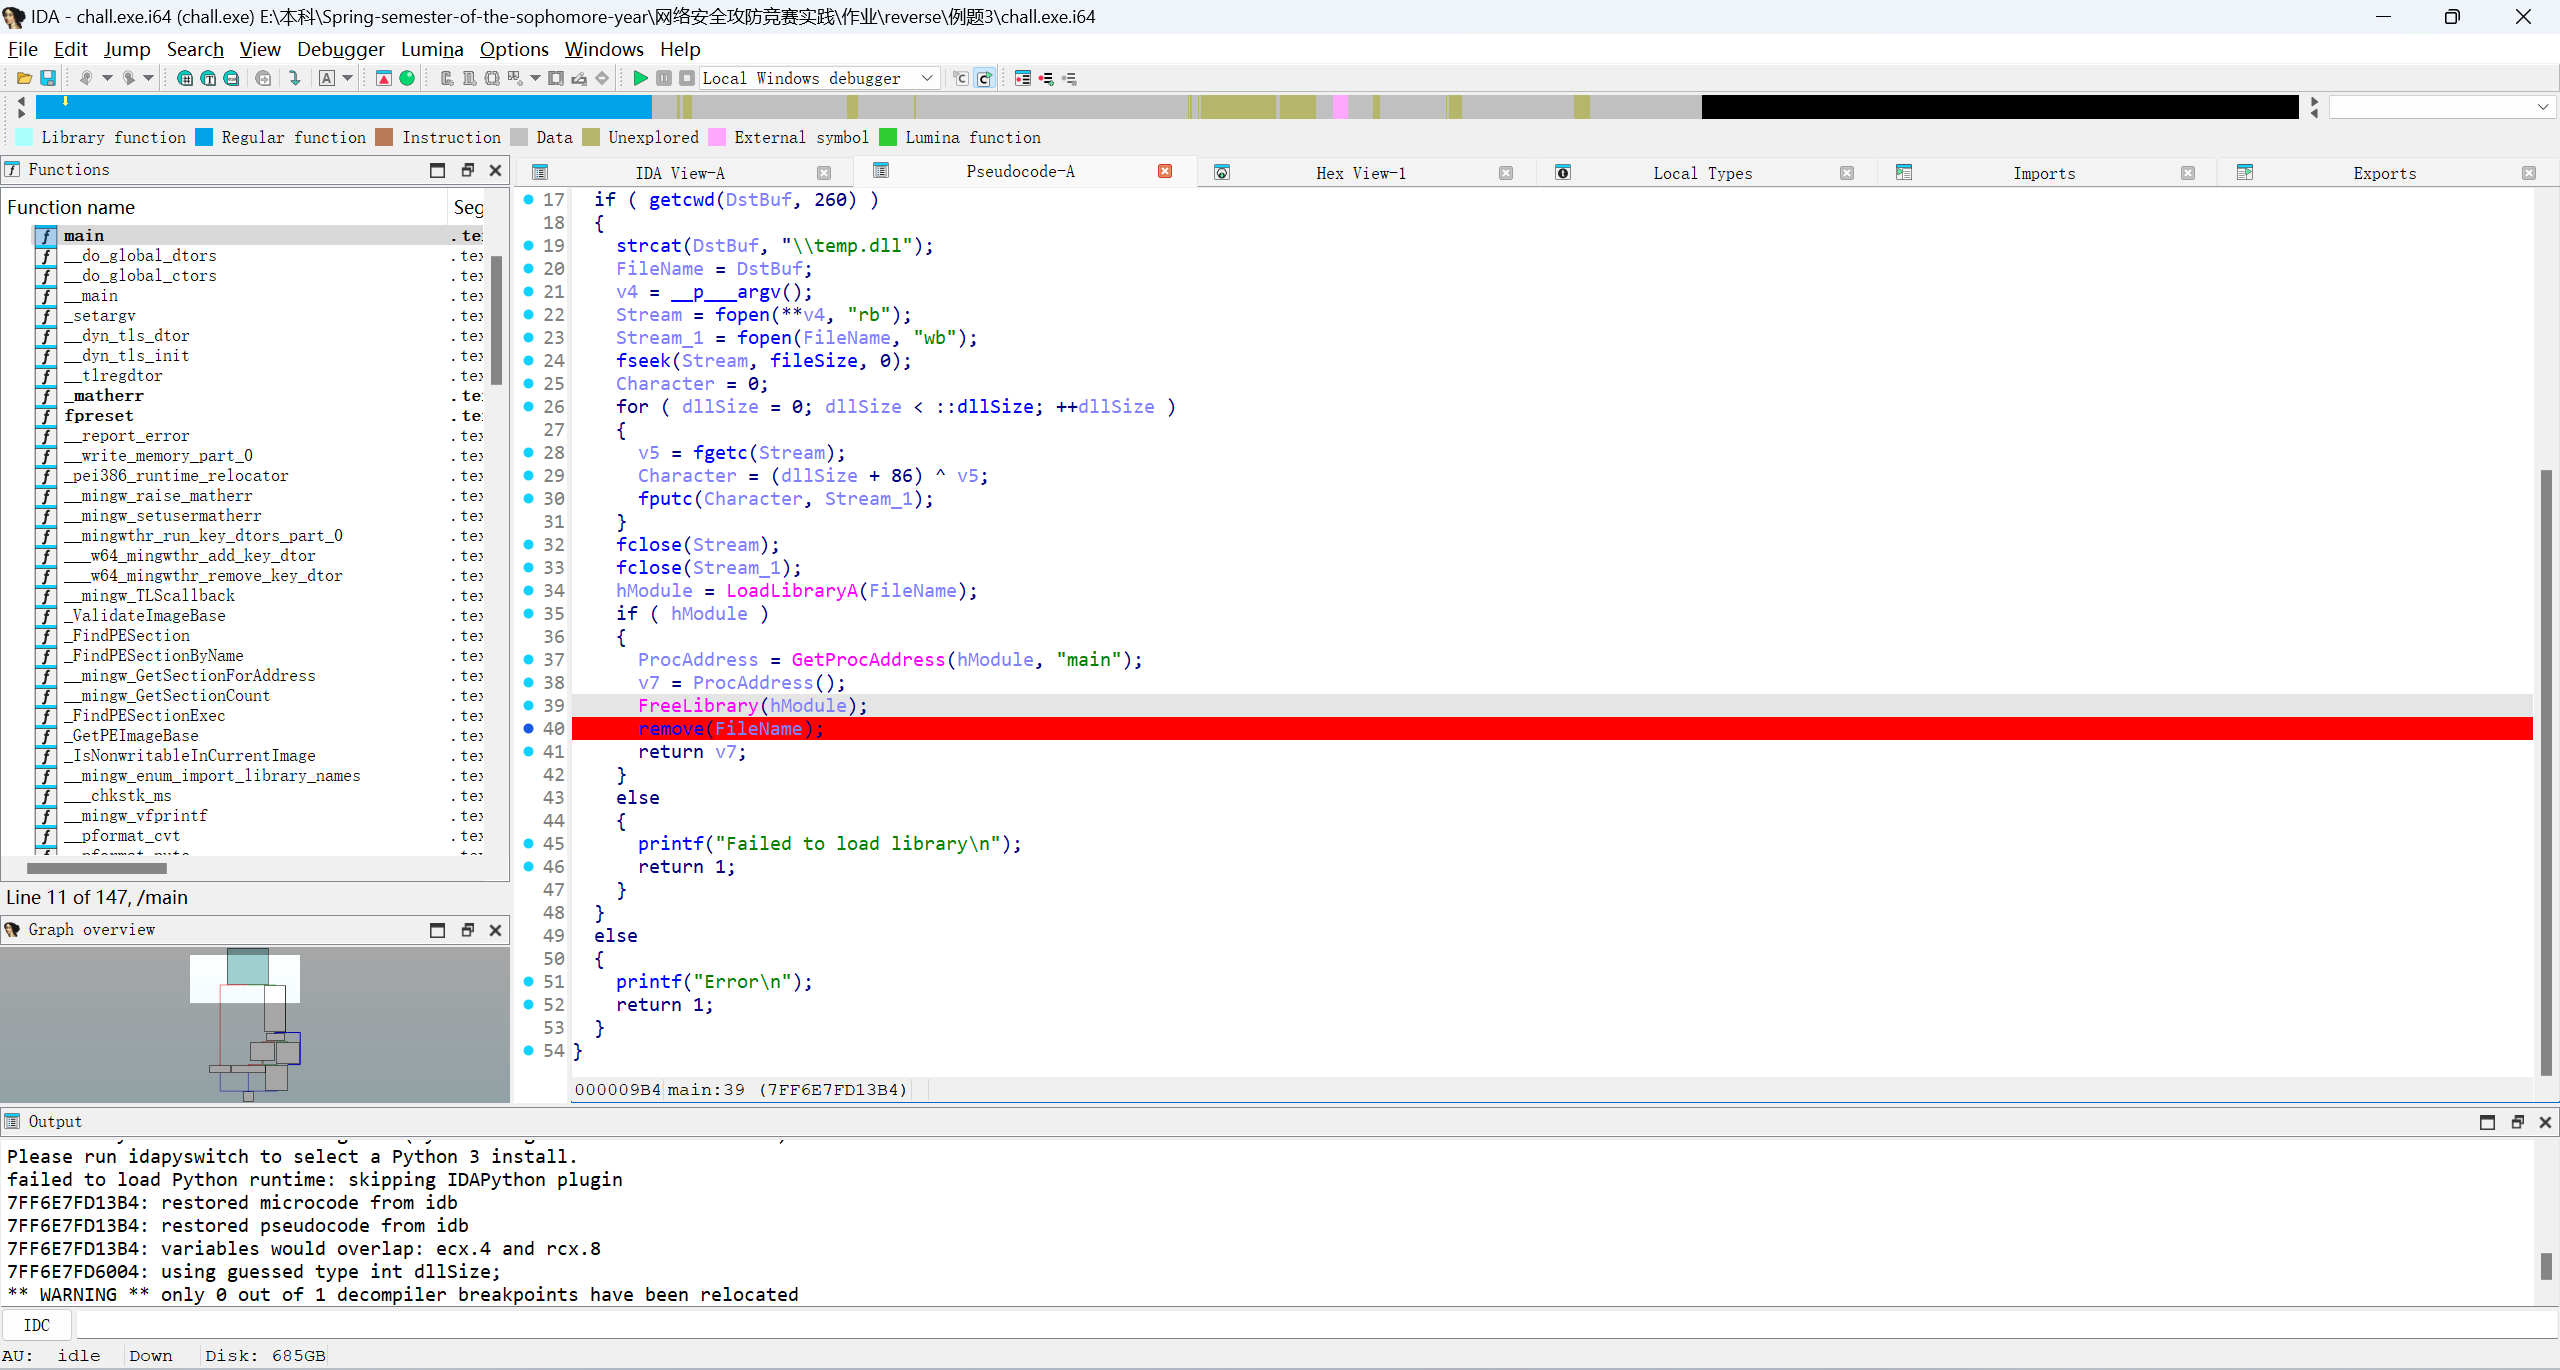
\includegraphics[width=0.95\textwidth]{3.3.png}
\end{figure}
\begin{figure}[H]
    \centering
    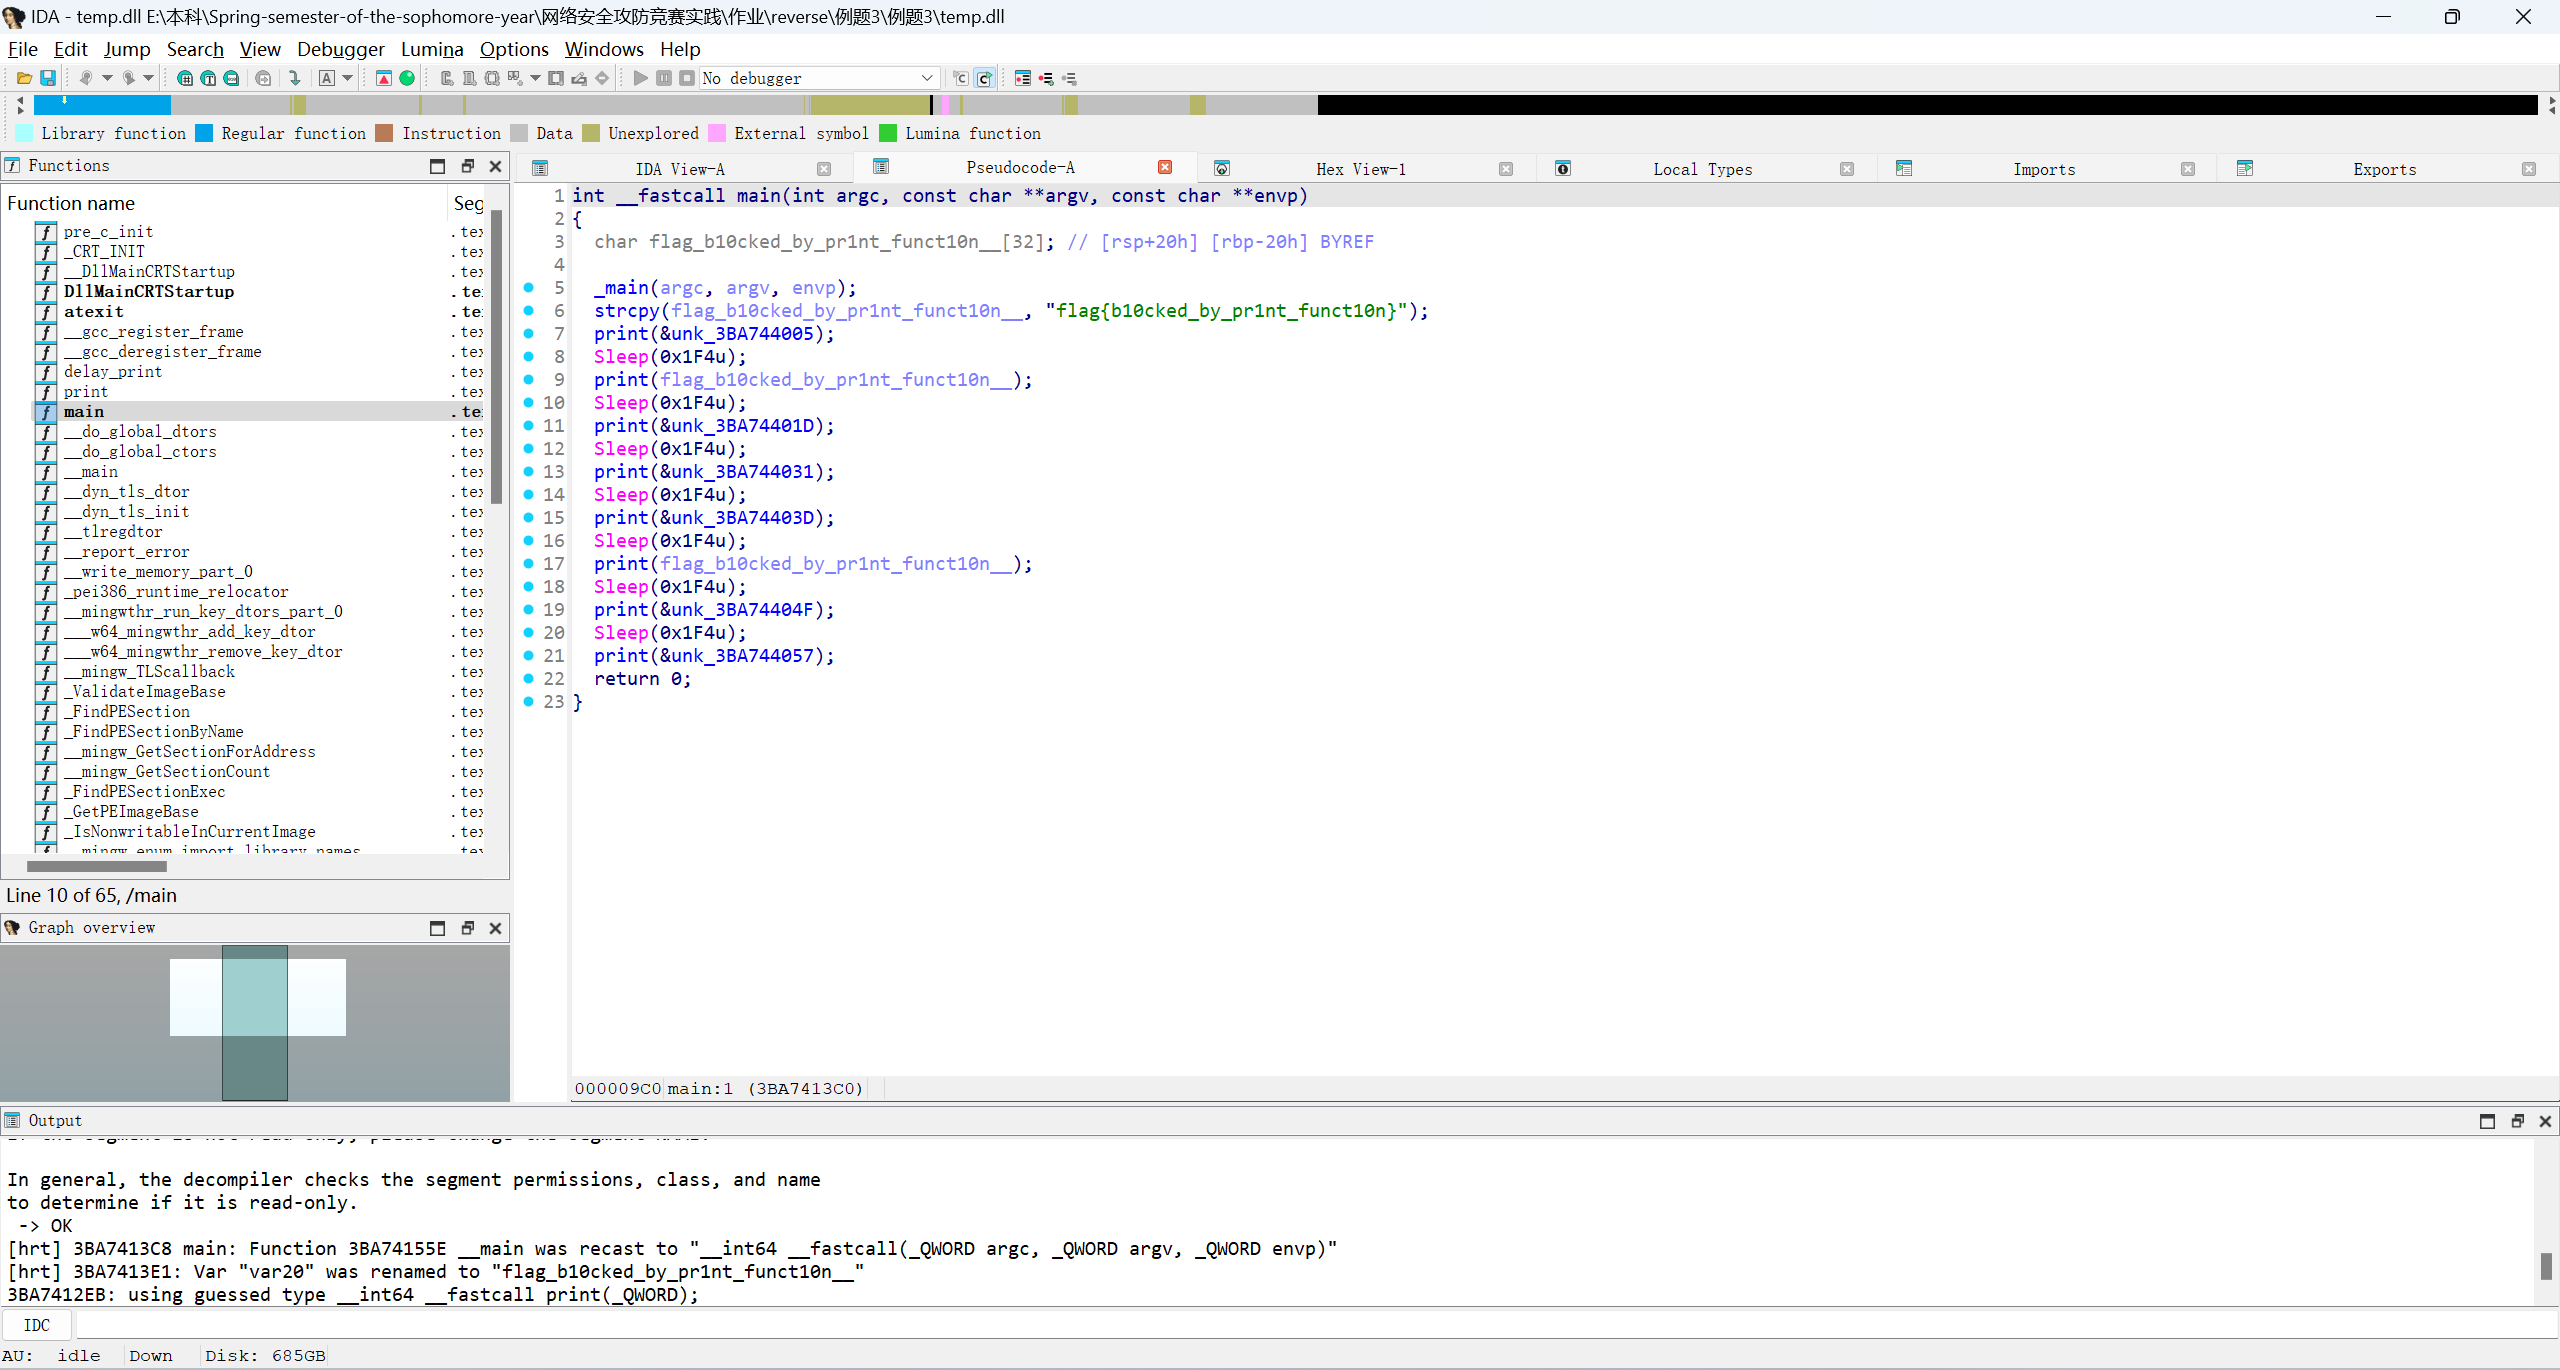
\includegraphics[width=0.95\textwidth]{3.4.png}
\end{figure}

\subsection{最终Flag}
\begin{center}
    \Large flag\{b10cked\_by\_pr1nt\_funct10n\}
\end{center}

\end{document}